%
% Unless otherwise indicated, the copyright in this material is 
% owned by Joerg Evermann. This material is licensed to you under the 
% Creative Commons by-attribution non-commercial license (CC BY-NC 4.0)}
%
\section*{Learning Goals}

After reading this chapter, you should be able to:
\begin{itemize}
   \item Explain different purposes for information visualization.
   \item Identify deceptive visualization techniques and avoid such techniques in your own visualizations.
   \item Understand different types of color palettes and be able to choose a color palette for a given visualization purpose.
   \item Understand the impact of color vision deficiency and its implications for creating meaningful visualization.
   \item Select a type of plot that is appropriate for a given purpose.
   \item Create different types of plots in R and Python, including customization of colors, axes, labels, and titles.
\end{itemize}

\section{Introduction}

Data visualization, the practice of transforming information into a visual context, has become an indispensable part of modern data analysis and communication. This field intersects art and science, requiring both creativity and analytical skills to convert complex data sets into comprehensible, insightful visual representations. The motivations for visualizing data are multifaceted. Primarily, it enhances understanding by simplifying complex information, making patterns, trends, and correlations more apparent than they would be in raw data. It also aids in storytelling, where data-driven narratives can be compellingly presented to a broad audience, regardless of their expertise in data analysis.

The purpose of visualization is to simplify, summarize and abstract complex information into an easy to understand format for human consumption, for understanding, persuasion or explanation, or for decision making. Visualizations can help to compare different objects or things, they can help identify trends, patterns, and relationships. In general, visualizations help in understanding data and gaining insight into a domain or pheonomenon.

The recent history of data visualization is marked by rapid advancements fueled by technology. In the last few decades, the advent of powerful computing and sophisticated software tools has revolutionized this field. Where once it was the domain of experts and specialists, data visualization has become accessible to a broader audience. Tools ranging from simple spreadsheet applications to advanced data visualization software have democratized the creation and interpretation of visual data. The rise of big data and machine learning has further escalated the importance of data visualization. As data sets have grown in size and complexity, the need for effective visualization tools has become more pronounced, leading to innovative methods and approaches. Interactive visualizations, real-time data mapping, and the use of virtual and augmented reality are some of the cutting-edge trends redefining how we see and interact with data today. This evolution continues as we find new ways to visually interpret the vast and growing ocean of data that characterizes the digital age.

Visualization is important because humans are very good at visual pattern recognition. In fact, humans are too good at this, as they tend to also recognize patterns where none exist. This makes it easy to deceive oneself or others with data visualizations. Hence, visualization should normally be undertaken with and supported by statistical data analysis to verify the existence of trends or differences.

\subsection*{Visual Discovery}

Visual discovery\index{Visual discovery} is the use of interactive visualization tools to uncover patterns, trends, and insights from data. This approach is a crucial aspect of modern data analysis, emphasizing the power of human visual perception. Visual discovery leverages the human brain's innate ability to process visual information rapidly. By translating complex data sets into graphical representations, it enables quicker and more intuitive understanding. Users can spot trends, outliers, differences, and patterns more easily than they could through rows of numbers or text.

Visual discovery is a highly iterative and dynamic process. Analysts rapidly create or change data visualizations, such as charts, graphs, and maps, to explore different aspects of the data. This interactivity allows for real-time exploration and analysis, making it easier to drill down into specifics, zoom out for a broader view or change the perspective one takes in examining data.

Visual discovery may be purely exploratory, without any prior knowledge by the data analyst, or it may seek to confirm or verify the beliefs or hypotheses that the data analyst has formed about the particular domain. However, even this confirmation is never final, but only a way to new insights and exploration. In this process, the analyst explores the data, forms some beliefs or hypotheses based on the exploration, tries to support it with a different visualization, and updates their beliefs or hypotheses based on the later visualization.

\subsection*{Declarative Visualization (''Storytelling'')}

In contrast to visual discovery, declarative visualization\index{Declarative visualization} is purpose-driven and aims to provide explanations to a particular audience. It is \emph{not} interactive or dynamic. Visualizations are intended to affirm or support a conclusion and to convince an audience or group of stakeholders. Information is not so much explored, as it is merely presented and explained in visualization. Declarative visualization is used to support decision making and is mainly static. 

\subsection*{Operational Visualization (Monitoring)}

In operational visualization, graphs and charts are used for supervision or monitoring of the operation of a system\index{Operational visualization}. They provide supervisors or controllers with a real-time view of the state of key system properties and are used to spot situations or trends that require intervention in the system's operation, that is, operational decision making. 

\subsection*{Quantitative Messages} 

Good visualizations are focused on the quantitative message they are intended to convey. For example, to present information about a time-series, that is, time-dependent behaviour of one or more variables, a line chart is a good type of visualization. However, that line chart would not be as useful to convey relative rankings of items or objects. For this purpose, a bar chart may be better suited. On the other hand, to describe part-whole relationships, a pie chart may be useful to show what part of the whole is contributed by its parts. Deviations from a mean or other standard, whether positive or negative, can be easily understood from a bar chart as well. To understand frequency distributions, one might use boxplots or histograms. Boxplots show median values, and measures of the ''spread'' or variability of the data. Histograms can show a one or two dimensional frequency distribution of values. To understand correlations of variables, a scatterplot is useful, where individual data points are plotted in a two or three dimensional coordinate system, often augmented with statistical information about their relationship. Finally, geographic information may use map data for visualization. This is sometimes called a ''cartogram''. Points may be overlaid on a map, or areas of a map may be colored or otherwise highlighted. In summary, it is important to consider the message to convey or the insight to be gained from a visualization when selecting the type of graph or chart.

\section{Honesty in Visualization}

For a number of reasons, it is easy to deceive with misleading visualizations. Humans are prone to see trends or patterns where none exist. A misleading visualization can exploit this propensity to suggest relationships between objects or variables that do not exist. Humans recognize some aspects of visualization better, earlier, and easier than others. For example, humans recognize the length of a line easier than the area of a surface, and recognize variations in color better than they interpret textual labels. A misleading visualization can exploit these cognitive effects to make the interpreter focus on particular, misleading aspects in the visualization. Finally, because visualizations are intended to abstract from the data itself and provide a summary, visualizations may not include sufficient information about the data or its processing to allow the reader to understand what is shown, making it easy to suggest interpretations that are misleading.

Here are some general guidelines for using visualizations:
\begin{itemize}
   \item Do not deceive the target audience
   \item Do not diminish or hide relationships or trends
   \item Do not exaggerate relationships or trends
   \item Do not obfuscate, confuse, or hide information
\end{itemize}

The term ''dark pattern'' has been coined to describe the opposite of best practices in a field; in this case practices that are intended to deceive, mislead, or frustrate others. There are many of such dark patterns in visualizations:

\begin{itemize}
	\item Use an inappropriate graph or chart type to hide or obfuscate relationships or trends. As noted above, different types of graph are suitable to convey different types of messages. An example is shown in Figure~\ref{fig:comparingpies} that illustrates that a bar or column chart is more useful for comparisons of objects than pie charts, so the use of a pie chart could hide or obfuscate trends that may otherwise be prominent.
	
\begin{figure}
\centering
\includegraphics[width=.8\textwidth]{screen7.png}

\scriptsize\url{https://en.wikipedia.org/wiki/Misleading_graph}
\caption{Comparing Pie Charts}
\label{fig:comparingpies}
\end{figure}

	\item \emph{Graph unrelated data to suggest non-existent relationships.} The viewer of a visualization expects that data that is graphed together has a meaningful relationship. Simply by graphing data together, the analyst suggests a relationship where none may exist.
	\item \emph{Scale multiple vertical axes to suggest correlations.} Scaling a graph with multiple vertical axes so that lines better align shows visual similarities that are not borne out by the data.
	\item \emph{Use confusing colors.} For example, a color palette whose perceived color differences do not map linearly to the actual differences in the data (that is, it is not ''\emph{perceptually uniform}'') may be misleading. For another example, using different shades of the same color for values that are very different will visually diminish the difference.
	\item \emph{Omit summary statistics.} For example, showing only the mean or median values, e.g. in a line or bar chart, omits the uncertainty in the data. It is better to also include error bars, information about quartiles or outliers in the chart to show variability or uncertainty, especially when there is significant uncertainty about differences or absolute values.
	\item \emph{Truncate or scale axes to hide or exaggerate trend.} Truncating or scaling axes leads to increased slopes of lines or perceived differences between points or levels. This exaggerates differences or trends. Figure~\ref{fig:truncated} shows an example of how small differences (right) can be exaggerated (left) in a bar chart. Similarly, Figure~\ref{fig:aspectratios} shows how scaling or the use of different aspect ratios can be used to visually exaggerate or diminish trends or relationships between variables.
\begin{figure}
\centering
\includegraphics[width=.85\textwidth]{screen3.png} \\

\scriptsize\url{https://en.wikipedia.org/wiki/Misleading_graph}
\caption{Truncated Axes}
\label{fig:truncated}
\end{figure}
\begin{figure}
\centering
\includegraphics[width=.85\textwidth]{screen4.png}

\scriptsize\url{https://en.wikipedia.org/wiki/Misleading_graph}
\caption{Scaling Axes and Aspect Ratios}
\label{fig:aspectratios}
\end{figure}
	\item \emph{Scale in multiple dimensions.} The relative change or difference should be represented by a single dimension only. For example, in a bar or column chart, only the height or length of bar/column should change, not its width or area as well. This issue is often connected to the use of 3-dimensional graphics. While visually appealing, they exaggerate the apparent visual area of a foreground object, as illustrated in Figure~\ref{fig:3dpie}. A related issue is the use of images in graphs, shown in Figure~\ref{fig:imagesgraphs}. In the improper scaling, the image is enlarged in two dimensions, visually suggesting a larger difference than there actually exists in the data.
\begin{figure}
\centering
\includegraphics[width=.8\textwidth]{screen6.png}

\scriptsize\url{https://en.wikipedia.org/wiki/Misleading_graph}
\caption{3D Pie Charts}
\label{fig:3dpie}
\end{figure}
\begin{figure}
\centering
\includegraphics[width=.75\textwidth]{screen1.png}

\scriptsize\url{https://en.wikipedia.org/wiki/Misleading_graph}
\caption{Scaling Multiple Dimensions}
\label{fig:imagesgraphs}
\end{figure}
	\item \emph{Plot cumulative growth to hide trend.} A cumulative trend will always a positive trend, even as the contribution of individual items decreases sharply.
	\item \emph{Use maps for non-geographic data.} Maps represent geographical area, rather than population or some other variables of interest. For example, coloring a map by voter preference visually overemphasizes thinly populated but large geographic areas.
	\item \emph{Use incomplete data (''cherry-picking'')}. This includes examples such as showing only the previous year's data, instead of data for the previous five years to hide a trend, showing quarterly data instead of weekly data to hide volatility, or showing every data for every second month instead of for every month to hide specific data points or trends. Figure~\ref{fig:omitted} shows an example of this dark pattern.
	\item \emph{Use invalid data.} When data is known to be unreliable, that is, its quality is low, its uncertainty may be high, and it has a large error rate, it is misleading to use it to convey a quantitative message. 
\begin{figure}
\centering
\includegraphics[width=\textwidth]{screen5.png}

\scriptsize\url{https://en.wikipedia.org/wiki/Misleading_graph}
\caption{Incomplete Data}
\label{fig:omitted}
\end{figure}

\end{itemize}	

The comics in Figure~\ref{fig:xkcd}, taken from the popular XKCD website\footnote{All XKCD comics are copyright by their creator (\url{www.xkcd.com}) and licensed under CC-BY-NC.} shows some of these visualization dark patterns in a humorous way. 

In summary, misleading charts and visualizations can be particularly problematic because they exploit the visual nature of human perception, making the deception less noticeable. It is crucial for both creators and consumers of data visualizations to be aware of these pitfalls and to approach data representation and interpretation with a critical eye.

\begin{figure}
\centering
\begin{subfigure}{.49\textwidth}
\centering
\includegraphics[width=\textwidth]{xkcd_convincing.png}
%\caption{Label your axes}
\end{subfigure}
\hfill
\begin{subfigure}{.49\textwidth}
\centering
  \includegraphics[width=\textwidth]{xkcd_self_description.png} 
%\caption{Use meaningful data}
\end{subfigure}
\hfill
\begin{subfigure}{.49\textwidth}
\centering
  \includegraphics[width=\textwidth]{xkcd_coronavirus_charts.png}
%\caption{Use related data}
\end{subfigure}
\hfill
\begin{subfigure}{.49\textwidth}
\centering
  \includegraphics[height=3in]{xkcd_curve_fitting.png}
%\caption{Do not mislead}
\end{subfigure}
\hfill
\begin{subfigure}{.49\textwidth}
\centering
  \includegraphics[height=2in]{xkcd_y_axis_2x.png}
%\caption{Choose Your Axes Meaningfully}
\end{subfigure}
\hfill
\begin{subfigure}{.49\textwidth}
\centering
  \includegraphics[width=.9\textwidth]{xkcd_extrapolating.png}
%\caption{Be Careful when extrapolating}
\end{subfigure}
\hfill
\begin{subfigure}{.49\textwidth}
\centering
  \includegraphics[width=\textwidth]{xkcd_linear_regression.png}
%\caption{Verify trends}
\end{subfigure}
\hfill
\begin{subfigure}{.49\textwidth}
\centering
  \includegraphics[width=.9\textwidth]{xkcd_log_scale.png}
%\caption{Use Appropriate Scales (XKCD)}
\end{subfigure}
 \\ 
\tiny \scriptsize{XKCD comics are copyright by their creator (\url{www.xkcd.com}) and licensed under CC-BY-NC}

\caption{Misleading Visualizations, Comics by XKCD}
\label{fig:xkcd}
\end{figure}


\section{Special Types of Data and Visual Analytics}

\subsection*{Streaming Data}

Visualizing streaming data, also known as real-time data visualization, involves the dynamic representation of data that is continuously updated as new data arrives. This type of visualization is essential in contexts where timely and rapid data interpretation is critical, such as in financial trading, or network monitoring. 

Streaming data presents some specific challenges for visualization. One of the primary challenges is managing the high velocity and volume of streaming data. The system must process and visualize data quickly enough to keep up with the incoming stream. Typically, only a limited window of data is available while older data is discarded. This means that, since the focus is on real-time data, it can be challenging to provide sufficient historical context for users to understand the current data in a broader temporal perspective. Moreover, due to the highly dynamic nature of the data, presenting streaming data in a way that is not overwhelming to the user is challenging. The visualization must strike a balance between providing enough detail and overloading the user with information, in particular information about changes, and also a balance between providing responsive graphs and overloading the user with such rapid changes they lose the ability to understand the data.

\subsection*{Spatial Data}

Visualizing geospatial or geographical data involves representing information that has a spatial component on a map or in a spatial context. While this type of visualization can be powerful for revealing patterns and insights related to location and geography, it presents some unique challenges. Geospatial data is often complex and multidimensional, encompassing not only locations but also attributes like time, elevation, population density, and more. Geospatial datasets can be very large, especially with the advent of satellite imagery, IoT (Internet of Things) sensors, and other sources of big data. Moreover, the granularity of physical space can range from very small areas of a few square meters to very large areas, such as provinces or states. For example, postal-code level data can produce very large data sets, even in small jurisdictions. 

A specific problem is the choice of areal unit to use for data analysis or visualization. For example, location data points can be aggregated by counties or districts, by postal code areas, by school districtcs or school intake areas, by police or fire service coverage, or many others. Each of these different areal units will lead to different data summaries and therefore also to different visualizations. Choosing the type of area to use as the basis for visualization can have a large impact on the insights gained or the messages conveyed to the audience. A simple example is shown in Figure~\ref{fig:maup} that shows how aggregate statistics depend on the type of areal unit or boundary.

\begin{figure}
\centering
\includegraphics[width=.5\textwidth]{Maup_rate_numbers.png} \\

\small \url{https://en.wikipedia.org/wiki/File:Maup_rate_numbers.png}
\caption{Different types of spatial divisions lead to different interpretations} 
\label{fig:maup}
\end{figure}

Another particular challenge with spatial data is mapping the three-dimensional Earth onto a two-dimensional surface. This mapping inevitably involves some form of projection, which can distort spatial relationships. Choosing an appropriate map projection that minimizes distortion for the specific data and use case is a critical challenge. There are many such projections\footnote{\url{https://en.wikipedia.org/wiki/Map_projection}}, that distort or leave undistorted various properties such as lengths, areas, or angles. Figure~\ref{fig:xkcdmaps} shows some of these issues in a humorous way.

\begin{figure}
\centering
\begin{subfigure}{.49\textwidth}
\centering
  \includegraphics[width=\textwidth]{xdcd_heatmap_2x.png}
\end{subfigure}
\hfill
\begin{subfigure}{.49\textwidth}
\centering
  \includegraphics[width=\textwidth]{xkcd_bad_map_projection_madagascator.png}
\end{subfigure}
\hfill
\begin{subfigure}{.49\textwidth}
\centering
  \includegraphics[width=\textwidth]{xkcd_bad_map_projection_the_greenland_special.png}
\end{subfigure}
\hfill
%\begin{subfigure}{.49\textwidth}
%\centering
  %\includegraphics[width=\textwidth]{xkcd_bad_map_projection_time_zones.png}
%\end{subfigure}
%\hfill
\begin{subfigure}{.49\textwidth}
\centering
  \includegraphics[width=\textwidth]{xkcd_state_word_map.png}
\end{subfigure} \\ 
\tiny \scriptsize{XKCD comics are copyright by their creator (\url{www.xkcd.com}) and licensed under CC-BY-NC}

\caption{Map Visualization Comics by XKCD}
\label{fig:xkcdmaps}
\end{figure}

\subsection*{Network and Graph Data}

Visualizing network or graph data involves representing entities as nodes and the relationships between them as edges in a graphical format. This type of visualization is crucial for understanding complex structures in various fields like social network analysis, biology, computer science, and more. Typically, nodes are represented as boxes, circles, or textual labels, while edges are represented as lines or curves. Directed graphs use arrowheads on lines or curves to indicate the directionality of an edge. 

As the number of nodes and edges increases, the visualization can quickly become a tangled mess, making it difficult to discern meaningful patterns or relationships. To effectively explore graph data interactive features like zooming, panning, and highlighting are essential. Graphs may also contain large sets of attributes for nodes and edges. Representing these attributes effectively without cluttering the visualization or overwhelming the viewer is challenging. Techniques like color coding, sizing, or shaping nodes and edges are commonly used techniques, but require careful design.

In densely connected networks, edges can overlap, and nodes can occlude each other, leading to a loss of information and making it difficult to trace relationships or identify individual elements. There exist many different ways to visually layout a graph to make it visually clear and easy to understand. 

One of the most commonly-used types of algorithms positions graph vertices based on the physical metaphors of attractive and repulsive forces, for example an imaginary system of physical springs, sometimes called a force-directed graph layout\index{Force-directed graph layout}. Adjacent vertices are modelled with an attractive force, while all vertices have a repulsive force. The graph layout algorithm then tries to produce a layout in which an overall energy function is minimized. Figure~\ref{fig:sna_viz} shows an example of such a graph layout.

Another commonly used graph layout algorithm is the simple circular layout, where nodes are arranged equidistantly around a circle with edges drawn as lines or arrows. Figure~\ref{fig:circular} shows an example this type of graph layout.

In an arc diagram, as shown in Figure~\ref{fig:arc}, the nodes are arranged on a straight line while edges are drawn as semicircles between nodes. In this layout, it is important to arrange the nodes to minimize the number of crossings of edge semicircles. 

A common type of layout for directed and acyclic graphs is the layered graph, typically layed out from top to bottom or from left to right. The layout begins at the root node or nodes, and increments the layer for each edge between adjacent nodes, as shown in Figure~\ref{fig:layered}.

\begin{figure}
\centering
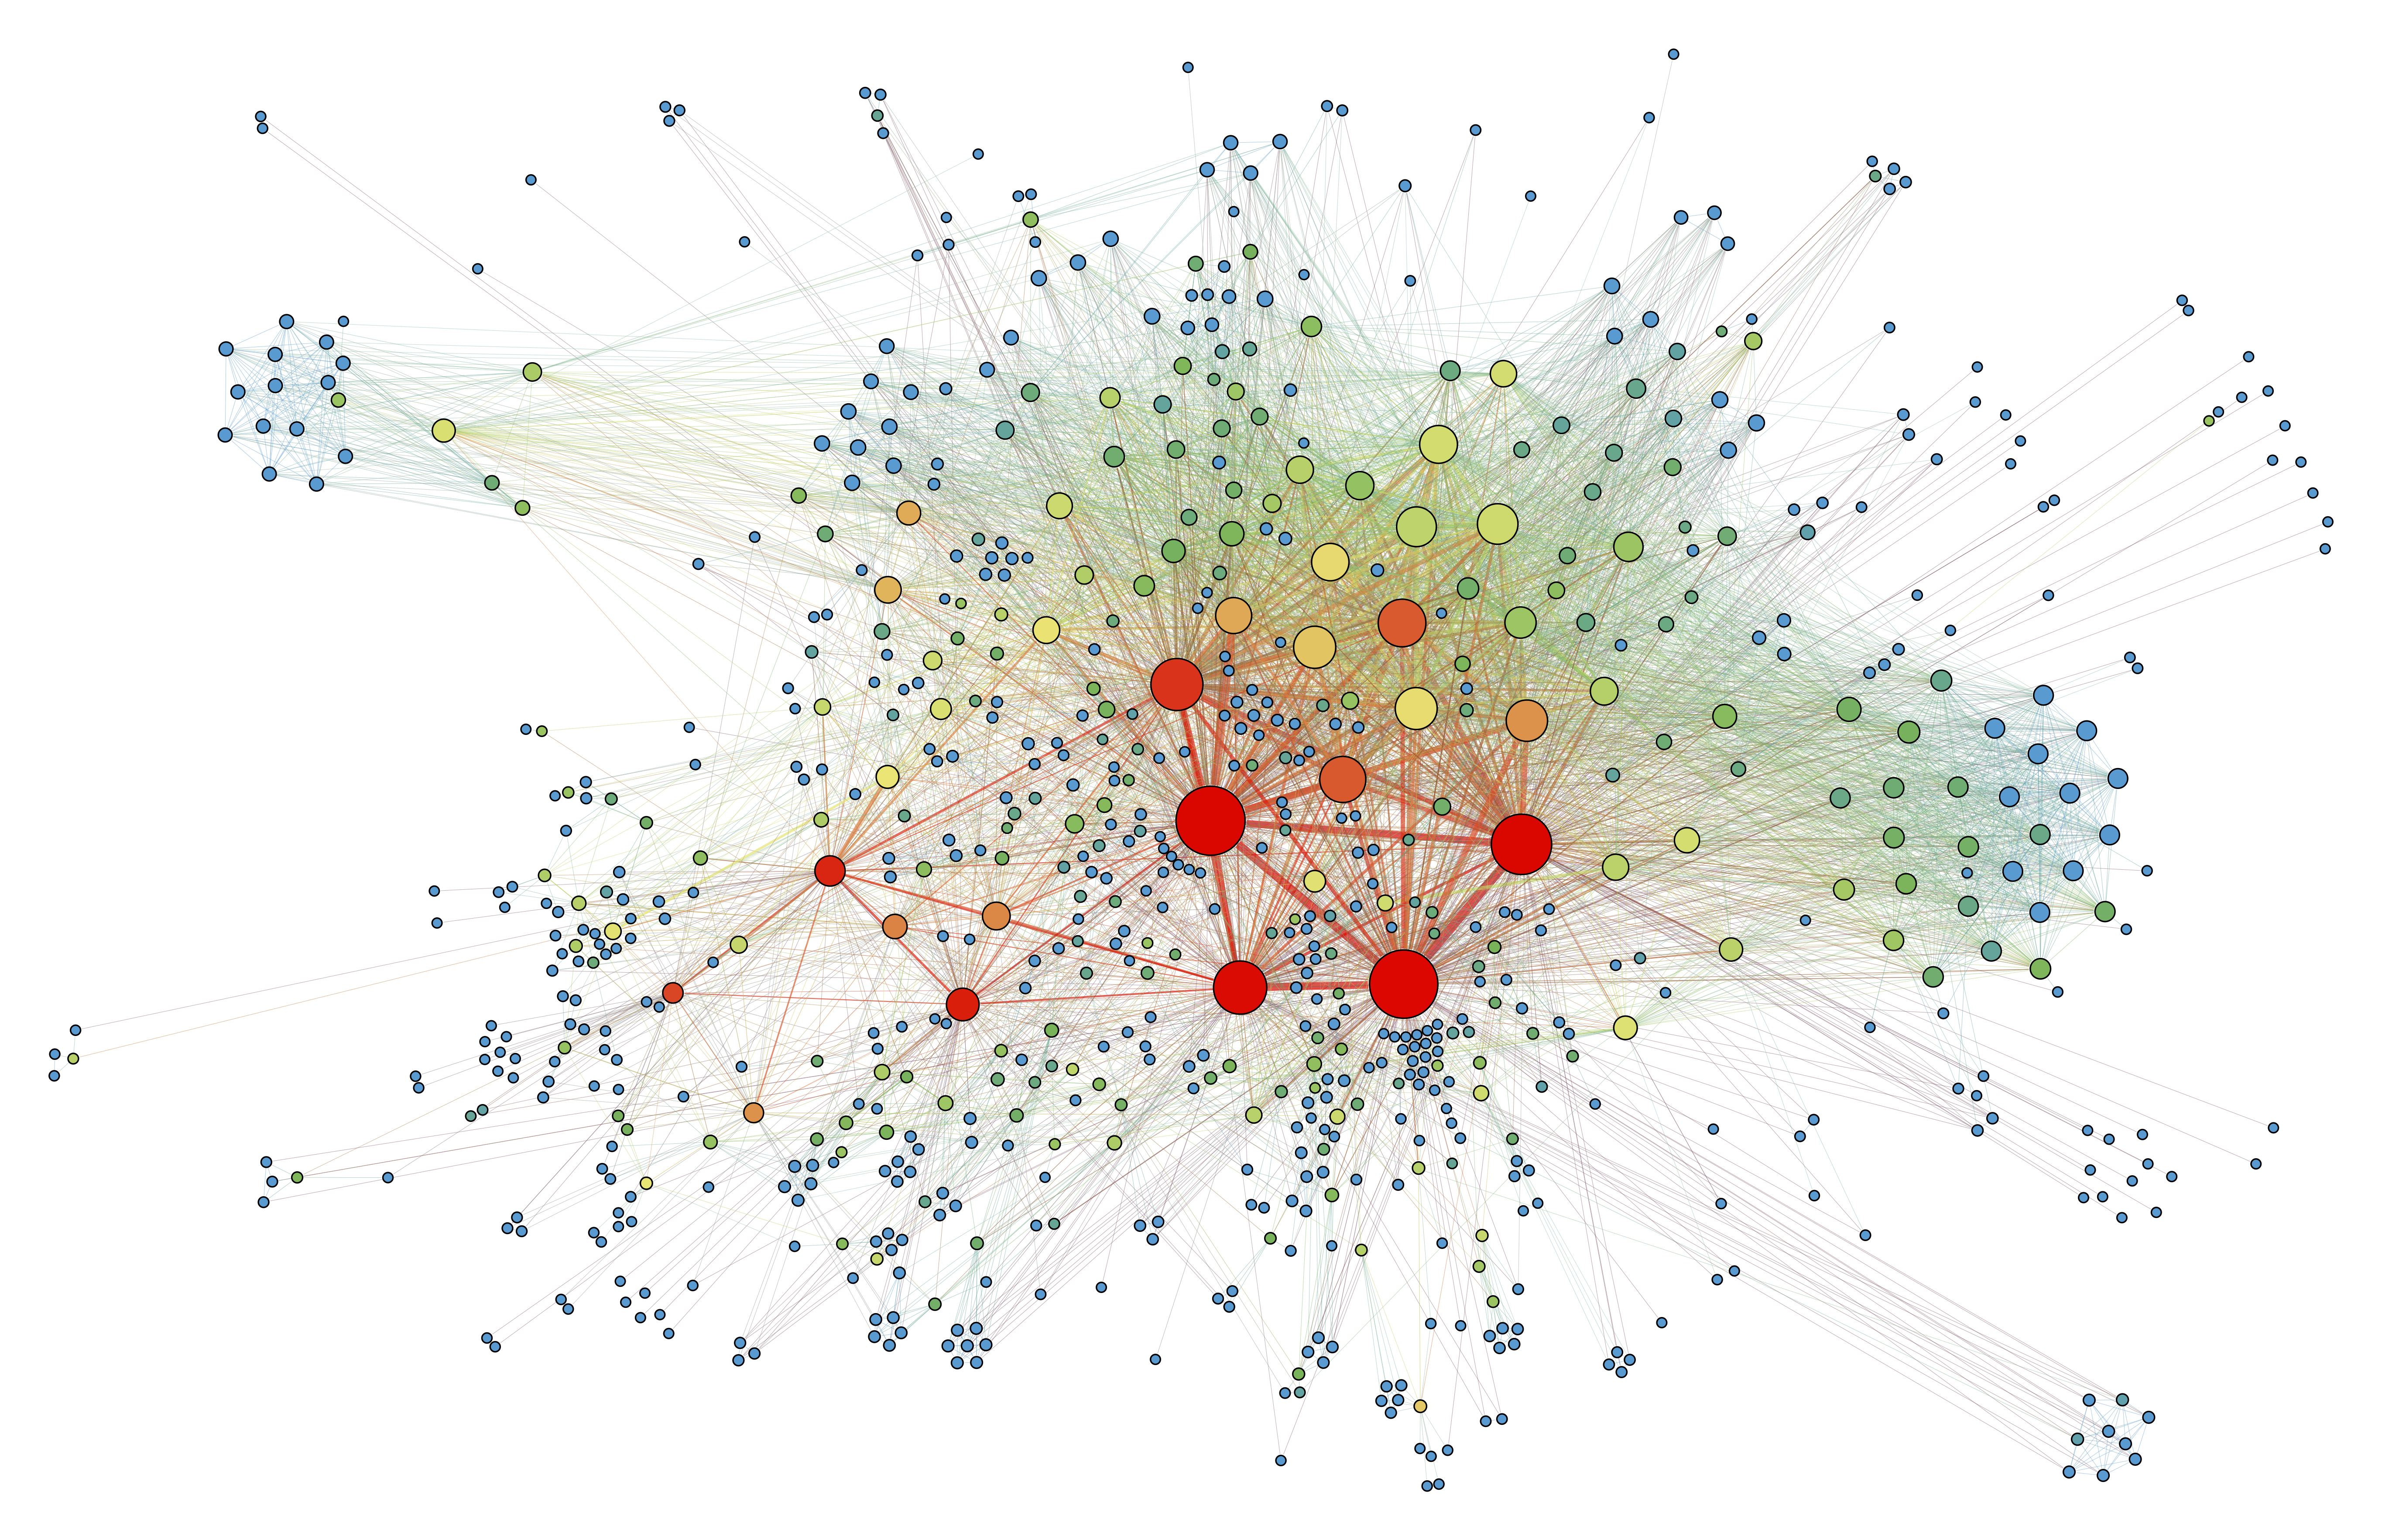
\includegraphics[width=.75\textwidth]{sna_viz.png} \\

\scriptsize \url{https://commons.wikimedia.org/wiki/File:SocialNetworkAnalysis.png}
\caption{Force-directed graph layout example} 
\label{fig:sna_viz}
\end{figure}

\begin{figure}
\centering
\includegraphics[width=.5\textwidth]{circular.png} \\

\scriptsize \url{https://commons.wikimedia.org/wiki/File:BGP_FSM_3.svg}
\caption{Circular graph layout example} 
\label{fig:circular}
\end{figure}

\begin{figure}
\centering
\includegraphics[width=.5\textwidth]{arc.png} \\

\scriptsize \url{https://commons.wikimedia.org/wiki/File:Goldner-Harary-linear.svg}
\caption{Arc graph layout example} 
\label{fig:arc}
\end{figure}

\begin{figure}
\centering
\includegraphics[width=\textwidth]{layered.png} \\

\scriptsize \url{https://commons.wikimedia.org/wiki/File:DC\%2B\%2B\_derivatives.svg}
\caption{Layered graph layout example} 
\label{fig:layered}
\end{figure}

%\noindent When assessing the quality of the graph layout, a number of considerations are important:

%\begin{itemize}
  %\item \emph{Number of crossings of lines or curves}. Such crossings are visually confusing and should be minimized. In fact, this is such an important criterion that graph theory has defined a planar graph as one that can be visualized in two dimensions without any line crossings. Another qual
  %\item \emph{Area of the graph}. Graphs should be drawn in the minimal amount of space while still being easy to read and understand.
  %\item \emph{Symmetries}. Being able to exploit symmetries in the underlying graph data and represent or highlight them in the graphical layout makes the graph visualization easier to understand. 
  %\item \emph{Shape homogeneity}. A particular problem when using node labels, e.g. for names or node attributes, is the size of the node shape in the graph visualization. It is preferrable to maintain equal size, despite differences in label length. Lines should have the lowest or an equal number of bends.
  %\item \emph{Angular resolution}. In graphs with many edges from nodes, it is important to draw lines in such a way that the edges can be clearly differentiated. This is very important in circular layouts, but also plays a large role in other types of graph layouts.
%\end{itemize}

\section{Color Palettes}

The use of color in data visualization is crucial, serving not only to enhance the visual appeal of a graphic but also to improve its clarity and interpretability. Color choices in data visualizations, determined by the selected color palettes, play a significant role in distinguishing different data points or categories, setting the tone of the presentation (for example, formal versus informal presentations), ensuring accessibility for viewers with color vision deficiencies, and enhancing the overall aesthetic appeal. Desirable characteristics of color palettes are:

\begin{itemize}
   \item \emph{Range of Values}: Colorful palettes are required when many different values have to be represented and distinguished.
   \item \emph{Perceptual Unformity}: The relative perceived differences between colors in the palette should mirror the relative differences in the data values represented by the colors.
   \item \emph{Robustness to Color Vision Deficiency}: Colour vision deficiency (CFD), colloquially called ''color blindness'' impacts almost 10\% of the population and must therefore be a consideration when choosing color palettes so that the data visualization can be properly perceived and interpreted by everyone.
   \item \emph{Consistency}: When using multiple plots, their color palette should be the same or at least consistent so as not to cause confusion in interpretation and require less effort for understanding by the reader.
   \item \emph{Aesthetic Appeal}: Finally, a colour palette should also be ''pretty''.
\end{itemize}

\subsection*{Types of Color Palettes}

Color palettes can be distinguished by the number of colours they use, and whether the colors span a continuous color space or are a discrete set. 

\subsubsection*{Sequential color palettes}

Sequential color palettes\index{Colour palette!sequential}, like the one in Figure~\ref{fig:sequential}, use a single color and vary the hue or depth of the color. They are best used for data that has an inherent order, as they clearly show progression or gradation. However, they are not suitable for data that lacks a natural ordering. The \emph{monochromatic color palette} is a special case of a sequential palette. This may be suitable when it is likely that the output will be printed on media without the use of color. 

\subsubsection*{Diverging color palettes}

Diverging color palettes\index{Colour palette!diverging}, like the one in Figure~\ref{fig:diverging} use two colors as anchors and use gradations either through white, as in Figure~\ref{fig:diverging}, or through black. They are ideal for emphasizing deviations from a median or mean value, or for highlighting extremes on either side of a critical midpoint. However, these palettes may be misleading if used for data without a meaningful center.

\subsubsection*{Spectral color palettes}

Spectral color palettes\index{Colour palette!spectral}, like the one in Figure~\ref{fig:spectral} use a variety of different colors without any implicit ordering. They are used to represent discrete categories without inherent ordering, and are useful for differentiating distinct groups of data. The downside is that they can become confusing with too many categories. 

Sequential and diverging color palettes may be \emph{discrete}\index{Colour palette!discrete}, like the ones shown in Figure~\ref{fig:palettes}, or \emph{continuous}\index{Colour palette!continuous}, while spectral palettes are always discrete.

\begin{figure}
\begin{subfigure}{\textwidth}
\centering
\includegraphics[width=.8\textwidth]{sequential.pdf}
\caption{Sequential color palette} 
\label{fig:sequential}
\end{subfigure}

\begin{subfigure}{\textwidth}
\centering
\includegraphics[width=.8\textwidth]{monochromatic.pdf}
\caption{Monochromatic color palette} 
\label{fig:monchromatic}
\end{subfigure}

\begin{subfigure}{\textwidth}
\centering
\includegraphics[width=.8\textwidth]{diverging.pdf}
\caption{Diverging color palette} 
\label{fig:diverging}
\end{subfigure}

\begin{subfigure}{\textwidth}
\centering
\includegraphics[width=.8\textwidth]{brewer.paired.pdf}
\caption{Spectral color palette} 
\label{fig:spectral}
\end{subfigure}

\caption{Types of Color Palettes}
\label{fig:palettes}
\end{figure}

\subsection*{Color Vision Deficiency}

The human eye contains three different types of color receptor cells, called ''S-cones'' that perceive the color blue, ''M-cones'' that perceive the color green, and ''L-cones'' that perceive the color red. Color vision deficiency (CVD)\index{Colour vision deficiency}\index{CVD|see{Colour vision deficiency}} is a biological impairment where some color receptor cells in the eye are missing, less frequent, or their function is diminished. In \emph{protanopia}\index{Protanopia}, the S-cones are missing or impaired, in \emph{deuteranopia}\index{Deuteranopia}, the M-cones are missing or impaired, and in \emph{tritanopia}\index{Tritanopia}, the L-cones are impaired. When all are missing or non-functional, one speaks of \emph{monochromatism}\index{Monochromatism}. CVD is a fairly common disability, afflicting approximately 1 in 12 men and 1 in 200 women, with an overall incidence rate in Canada of more than 5\%.

To show the different types of color deficiencies, consider the images in Figure~\ref{fig:cvd}. Figure~\ref{fig:cvd1} shows the original image as it is perceived by a person who does not suffer from CVD. The remaining four images show how the photo appears to persons with different types of CVD.

\begin{figure}
\centering
\begin{subfigure}{.75\textwidth}
\centering
\includegraphics[width=\textwidth]{photo.jpg} \\

\scriptsize Copyright Memorial University of Newfoundland 
\caption{Original Image (MUN Faculty of Education Class Room)} 
\label{fig:cvd1}
\end{subfigure}
\hfill
\begin{subfigure}{.49\textwidth}
\centering
\includegraphics[width=\textwidth]{desaturate_photo.jpg}
\caption{Monochromatism} 
\label{fig:cvd2}
\end{subfigure}
\hfill
\begin{subfigure}{.49\textwidth}
\centering
\includegraphics[width=\textwidth]{protan_photo.jpg}
\caption{Protanopia} 
\label{fig:cvd3}
\end{subfigure}
\hfill
\begin{subfigure}{.49\textwidth}
\centering
\includegraphics[width=\textwidth]{deutan_photo.jpg}
\caption{Deuteranopia} 
\label{fig:cvd4}
\end{subfigure}
\hfill
\begin{subfigure}{.49\textwidth}
\centering
\includegraphics[width=\textwidth]{tritan_photo.jpg}
\caption{Tritanopia} 
\label{fig:cvd5}
\end{subfigure}
\hfill
\caption{Simulated Color Vision Deficiencies}
\label{fig:cvd}
\end{figure}

Realizing the prevalence and the effects of CVD means that the color palette that is chosen for data visualization should be interpretable for and lead to the same interpretation even for readers with CVD. For example, the Viridis color palette available in many visualization software packages was designed with CVD readability in mind. Compare the popular ''Color Brewer Paired'' palette in Figure~\ref{fig:paired} to the Viridis palette in Figure~\ref{fig:viridis}. The figures show that the Viridis palette is readable and interpretable with any CVD condition, whereas the Paired palette is not because some colors cannot be distinguished under various CVD conditions.

\begin{figure}
\centering
  \includegraphics[width=.75\textwidth]{brewer.paired.cvd.pdf}

\caption{Colourbrewer ''Paired'' Colour Palette}
\label{fig:paired}
\end{figure}

\begin{figure}
\centering
  \includegraphics[width=.75\textwidth]{viridis.plot.pdf}

\caption{Viridis Colour Palette}
\label{fig:viridis}
\end{figure}

In summary, the thoughtful application of color in data visualization is not merely an artistic decision but a strategic one. It influences how effectively the data is communicated and understood, ensuring that visualizations are not only informative and accurate, but also inclusive and engaging to a diverse audience.

\FloatBarrier

\section{Common Types of Plots}

Depending on the number of variables to visualize, whether they are discrete or continuous, and the quantitative message to convey, different types of plots may be chosen. While the list of plot types presented here is not comprehensive, and new ways of visualizing data are constantly being invented, these are widely used plot types that are available in most visualization software packages and can be created with little effort.

\begin{itemize}
   \item Plots for One Variable
   \begin{itemize}
      \item Continuous 
      \begin{itemize}
		\item {\bf Area}: Degree of change over time, or relationship of parts to aggregate
		\item {\bf Density, Dot, Frequency, Histogram}: Show frequency distribution of data
	  \end{itemize}
	  \item Discrete
		\begin{itemize}
		  \item {\bf Bar}: Connections among individual things, compare items of different groups
		  \item {\bf Pie}: Relationships of parts to aggregate
		\end{itemize}
    \end{itemize}
    \item Plots for Two Variables
    \begin{itemize}
       \item Both Continuous
			\begin{itemize}
			  \item {\bf Point}: Connections among numeric values, show multiple groups of data
			  \item {\bf Lines, Local Regression}: Relationships/correlations among multiple data series or over time
			  \item {\bf Text / Label}: Frequency of labels in content/document
			\end{itemize}
	   \item One Discrete, One Continuous
			\begin{itemize}
			  \item {\bf Column}: Correlations among things or information changes over time
			  \item {\bf Box, Dot, Violin}: Compare distributions between many groups, display spread and skew of data
			\end{itemize}
	   \item Both Discrete
			\begin{itemize}
				\item {\bf Points/Counts}: Magnitude of counts
				\item {\bf Jitter}: Plots of data points
			\end{itemize}
		\item Distributions of Two Variables
			\begin{itemize}
				\item {\bf Bin2D, Density2D, Hex}: Shows frequency of values over two continuous variables
			\end{itemize}
	\end{itemize}
	\item Plots for Three Variables
	\begin{itemize}
		\item Continuous
			\begin{itemize}
				\item {\bf Contour, Raster and Tile}: Shows relationships among three data series
			\end{itemize}
	\end{itemize}
	\item Visualizing Errors and Uncertainty
	\begin{itemize}
		\item Give a general idea of how precise a value is, or how far a value might be from the true value
		\item Typically used to augment a given visualization
		\item Common Visualization Styles:
			\begin{itemize}
			  \item Crossbar
			  \item Errorbar
			  \item Range (line, point)
			\end{itemize}  
	\end{itemize}
\end{itemize}

\section{Graphics Libraries and Frameworks}

\subsection*{R}

The R software system offers several powerful data visualization packages, each with unique features and strengths. Among the most prominent are ggplot2, Plotly for R, ggvis, and Shiny, which collectively cater to a wide range of visualization needs.

At the forefront is \emph{ggplot2}, a package based on the Grammar of Graphics, which provides a coherent system for describing and building graphs. Its strength lies in its ability to create complex, multi-layered graphics with a syntax that is both powerful and expressive. ggplot2's approach allows users to build plots layer by layer, making it easier to handle and modify the components of a graphic. Its extensive customization options and the ability to handle a wide variety of graphical forms make it popular for static graphics.

\emph{Plotly for R} integrates the functionality of the Plotly JavaScript library into R, enabling the creation of interactive, web-based graphs. This package extends the interactive capabilities of R visualizations, allowing users to produce graphics that can be zoomed, panned, and hovered over to reveal additional information. Its integration with R makes it a popular choice for adding an interactive element to data presentations, bridging the gap between static and dynamic visualizations.

\emph{ggvis}, another package in the R visualization landscape, combines the concepts of ggplot2 with the interactivity of the web. It is designed to integrate well with R's reactive programming package, Shiny, and the dplyr package, enabling a smooth workflow for interactive data exploration. ggvis focuses on web-based, interactive visualizations, providing a syntax similar to ggplot2 but with additional capabilities to interactively change the data display and explore data in real-time.

\emph{Shiny}, distinct from the traditional visualization packages, is an R package for building interactive web applications. It allows users to turn their analyses into interactive web applications without requiring HTML, CSS, or JavaScript knowledge. Shiny applications have the power to not only display complex visualizations but also to interact with the user, making it possible to dynamically change the data, the types of plots, filters, and other aspects of the visualization based on user input. This interactivity makes Shiny particularly useful for creating data dashboards, where users need to explore and interact with data in a flexible manner.

Together, these packages provide R users with a comprehensive toolkit for creating static and interactive visualizations. From detailed and layered static plots with ggplot2 to dynamic, user-driven applications with Shiny, the R ecosystem enables a vast array of data visualization possibilities, catering to both simple and complex, interactive data exploration and presentation needs.

\subsection*{Python}

The Python programming environment also offers a rich landscape of data visualization packages, each tailored to different needs and preferences.

\emph{Matplotlib} is the foundational library for data visualization in Python, offering a wide array of functionalities to create static, animated, and interactive plots. It is highly customizable and capable of creating virtually any type of chart or graph. The versatility of Matplotlib allows for detailed control over plot elements, but this can also lead to more complex code for intricate visualizations.

\emph{Seaborn} builds on Matplotlib and simplifies the creation of beautiful, informative statistical graphics. It integrates closely with Pandas, a data manipulation library in Python, and provides a high-level interface for drawing attractive and informative statistical graphics. Seaborn's strength lies in its ability to create complex visualizations like heatmaps, time series, and violin plots with relatively straightforward commands.

\emph{Plotnine} is inspired by R's ggplot2 library and brings the Grammar of Graphics to Python. It offers a similar layer-based approach to visualization, making it a familiar choice for users transitioning from R to Python. Plotnine is particularly effective for creating complex, multi-layered graphics with a syntax that emphasizes the declarative nature of the visualization process.

\emph{Plotly Express} is a high-level interface for the Plotly library, designed to make it easy to create complex, interactive, and beautifully rendered visualizations. It offers a simple syntax for creating a wide variety of chart types and is particularly adept at handling large and complex datasets. Plotly Express's strength lies in its integration with Dash, another Plotly product, for building interactive web applications.

\emph{Plotly Graph Objects} is the lower-level interface of the Plotly library, providing more granular control over the visualization elements. It's ideal for users who need to create highly customized visualizations or who require fine-tuning beyond what Plotly Express offers.

\emph{Plotly Dash} is a framework for building interactive web applications with Python (and R and Julia). Dash is unique in its ability to create richly interactive, web-based data visualizations and dashboards without requiring advanced knowledge of web development. It integrates seamlessly with Plotly's suite, allowing for the creation of sophisticated data visualization interfaces.

\emph{Bokeh}, another prominent Python library, excels in creating interactive and real-time streaming visualizations. It is particularly well-suited for web-based dashboards and applications, offering both simplicity in creating complex interactive plots and the power to handle streaming datasets.

In summary, Python's ecosystem for data visualization is diverse and robust, ranging from Matplotlib's comprehensive capabilities for static plots to the interactive and web-based functionalities of Plotly and Bokeh. Each library offers unique strengths, whether it be in creating complex statistical visualizations, interactive web applications, or real-time data streams, catering to a wide range of data visualization needs and preferences.

\subsection*{JavaScript/Web}

JavaScript, being the standard language of web development, boasts several powerful data visualization libraries that are integral for creating interactive and dynamic visualizations on the web. Among these, D3.js, Chart.js, and Google Charts are particularly noteworthy, each with their unique capabilities and strengths.

\emph{D3.js} stands out as the most sophisticated and flexible JavaScript library for data visualization. Its core strength lies in its ability to bind arbitrary data to a Document Object Model (DOM), and then apply data-driven transformations to the document. D3 allows for extremely detailed and sophisticated visualizations by giving developers direct control over the SVG or HTML output. This level of control enables the creation of complex, interactive, and highly customizable visualizations. However, this power comes with a steep learning curve and can be overkill for simpler visualizations.

\emph{Chart.js} is a more lightweight and user-friendly alternative, specifically designed for creating simple yet beautiful and interactive charts. It uses HTML5 Canvas for rendering, which makes it efficient in terms of performance. Chart.js supports a variety of chart types, including bar, line, pie, radar, and more, all of which are responsive and mobile-ready by default. Its simplicity and ease of use make it a popular choice for developers who need to implement standard charts quickly and without the complexity of D3.js.

\emph{Google Charts} provides an even simpler way of incorporating charts into web pages. It offers a wide array of chart types and is particularly known for its integration with other Google services, like Google Spreadsheets. Google Charts is designed to be easy to use, and it handles a lot of the heavy lifting behind the scenes, such as drawing the charts, which makes it an appealing option for users who prefer a more straightforward and less code-intensive approach. The downside is that it offers less customization compared to D3.js and is reliant on external Google services, which might raise privacy concerns or issues with data control.

Each of these libraries serves different needs within the web development and data visualization community. D3.js is ideal for creating complex, interactive visualizations where control and customization are paramount. Chart.js offers a balance between simplicity and functionality, suitable for standard web-based charts. Google Charts, with its ease of use and integration with Google products, is excellent for straightforward visualizations where ease of implementation is a priority. The choice among these libraries largely depends on the specific requirements of the project, the complexity of the visualizations needed, and the developer's proficiency with JavaScript and web technologies.

\section{Mapping Data to Plot Elements}

Creating a basic visualization in two dimensions, such as  bar chart, a line chart, or a bubble chart, means that data variables or data series must be mapped to visualization elements. This is the core of the visualization task, and the most fundamental choice the data analyst has to make. Table~\ref{tab:elements} shows plot elements that data variables can be mapped to. In principle, a different data variable can be mapped to each of these, resulting in potentially being able to represent more than a dozen variables in one diagram. However, in practice, the number of concurrent variables to represent should be limited to no more than 3, in order for the visualization to remain interpretable and not to require too much cognitive effort on the part of the reader. The next sections show examples of mapping different variables to different plot element. 

\begin{table}[h]
\centering
\renewcommand{\arraystretch}{1.25}

\begin{tabular}{l} \hline
X, Y, Z axes \\
Colour (of points, lines, areas, shapes) \\ 
Transparency (''alpha'') \\
Patterns (within areas, shapes) \\
Size, Weight/Width (of points and lines) \\
Shape, Style (of points and lines) \\ \hline
\end{tabular}
\caption{Plot elements that can be mapped to data variables}
\label{tab:elements}
\end{table}

\section{Visualization in R using ggplot2}

This section provides an introduction to data visualization using the ggplot2 library in R. The example dataset for this section is the Fuel Consumption Ratings for battery electric vehicles, provided the Government of Canada through its Open Government Portal\footnote{\scriptsize\url{https://open.canada.ca/data/en/dataset/98f1a129-f628-4ce4-b24d-6f16bf24dd64}}. At the time of writing, the dataset was last updated on October 10, 2023. The dataset contains the variables shown in Table~\ref{tab:fueldata}.

\begin{table}[h]
\centering
\renewcommand{\arraystretch}{1.25}

\begin{tabularx}{\linewidth}{|l|l|X|} \hline
  {\bf Column} & {\bf Data Type} & {\bf Definition} \\ \hline \hline
  Make & Discrete & Manufacturer \\ 
  Model & Discrete & Model name\\
  Year & Numeric & Model year \\
  Category & Discrete & Small, Midsize, Large, Pickup, SUV, Station Wagon, etc. \\
  City & Numeric & Consumption in l/100km equiv. \\
  Hwy & Numeric & Consumption in l/100km equiv. \\
  Comb & Numeric & Consumption in l/100km equiv. \\
  Range & Numeric & Driving range in km \\ \hline
\end{tabularx}
\caption{Fuel efficiency data set variables}
\label{tab:fueldata}
\end{table}

\noindent Reading and preprocessing the data is straightforward in R, shown in the following code block:

\begin{Rcode}
# Load tidyverse package
library(tidyverse)

# Read the data set to a Tibble
data <- read_csv('https://evermann.ca/busi4720/fuel.csv')

# Ensure vehicle category is a factor (categorical)
data$Fuel <- as.factor(data$Fuel)
\end{Rcode}

\noindent Next, load the required graphics libraries. A number of extensions to the core ggplot2 library have been developed to provide additional capabilities, such as radar plots, pattern fills, providing more control over scales and axes, etc.

\begin{Rcode}
library(ggplot2)
library(ggpattern)
library(ggstream)
library(ggsci)
library(scales)
library(ggrepel)
library(ggradar)
\end{Rcode}

The core \texttt{ggplot()} function can be used in a dplyr pipeline and accepts the processed data tibble. The core argument to \texttt{ggplot()} is the ''\emph{aesthetic}'' that maps plot elements to data variables. The actual plots themselves are then added through the use of various ''\texttt{geoms}''. Such geoms respresent commonly used plot types. The geoms ''inherit'' the aesthetic specified in \texttt{ggplot()} and can add to it by including more variables mapped to different plot elements. More than one geom can be added to a plot, allowing the analyst to overlay plot types or combine plots for multiple data series or data sets. The final graph can be saved in a variety of different image formats. The following examples are intentionally kept simple and are not intended to show the full capabilities of the ggplot package. Many of the functions used below have a multitude of options to customize the output and a wide variety of ways, but this section focuses on the default visualizations they produce.

The first example below introduces the histogram geom. Histograms\index{Plot!Histogram} show the count of values in a certain range. The \texttt{ggplot()} function's aesthetic maps the ''Range'' variable of the data tibble to the x axis of the plot. The argument to the \texttt{geom\_histogram()} function indcates that 50 bins should be formed, i.e. the data is divided in 50 separate regions for counting and plotting.

\begin{Rcode}
data |> 
  ggplot(aes(x=Range)) + 
    geom_histogram(bins=50)
\end{Rcode}

The \texttt{ggsave()} function saves the last plot in a file with the specified height and width. The function attempts to automatically determine the output format, such as JPEG or PNG raster images, PDF files, etc. from the file name ending. See the manual (\texttt{?ggsave}) for further options. 

\begin{Rcode}
ggsave("histogram.pdf", height=5, width=7.5, units='in')
\end{Rcode}

\begin{center}
\includegraphics[width=.8\textwidth]{histogram.pdf}
\end{center}

A density plot\index{Plot!Density} using the \texttt{geom\_density()} function, is similar to a histogram in that it indicates the frequency of values. However, a density plot shows a continuous \emph{probability distribution} of the data values, and as such the vertical axis is limited in range between 0 and 1. The \texttt{kernel} option for the \texttt{geom\_density} geom specifies how the line is smoothed to produce the curve in the plot below. 

\begin{Rcode}
data |> 
  ggplot(aes(Range)) + 
    geom_density(kernel='gaussian', fill='lightblue')
\end{Rcode}

\begin{center}
\includegraphics[width=.8\textwidth]{fuel.density.simple.pdf}
\end{center}

%The example below adds a number of elements to the basic density plot. The function \texttt{labs()} allows specification of labels for all plot elements. The \texttt{geom\_vline()} geoms add vertical lines. Note that these geoms do not receive the data from the pipe, but the data is specified using the \texttt{data} argument. The aesthetics of a vertical line map the x axis intercept to a data variable. Different line types are used for the different lines. The \texttt{annotate()} function adds text annotations to the plot. Each annotation prints a label at a set of x and y coordinates in the plot, with a specific size and horizontal justification. For example, \texttt{hjust=0} means the text is left-justified. Consult the documentation for further details. 

%\begin{Rcode}
%# Prepare summary statistics

%mean_v <- e.clean |>
   %summarize(mean_v = mean(Range), 
             %median_v = median(Range), 
             %lower95=quantile(Range, .025), 
             %upper95=quantile(Range, .975), 
             %maxdensity = max(density(Range)$y))

%e.clean |>
  %ggplot(aes(Range)) + 
    %geom_density(kernel='gaussian', 
                 %fill='lightblue') + 
    %labs(x = 'Range (km)', 
         %y = 'Proportion of Vehicles', 
         %title='Density Plot - Electric Vehicle Range', 
         %subtitle='Years 2012 to 2024', 
         %caption='Lower and Upper 95 percentile, \
                  %median and mean') +
    %geom_vline(data=mean_v, 
               %aes(xintercept=mean_v), 
               %linetype='dashed') +
    %geom_vline(data=mean_v, 
               %aes(xintercept=median_v), 
               %linetype='dotdash') +
    %geom_vline(data=mean_v, 
               %aes(xintercept=lower95), 
               %linetype='dotted') +
    %geom_vline(data=mean_v, 
               %aes(xintercept=upper95), 
               %linetype='dotted') + 
	%annotate('text', 
	   %label=paste(' L95=\n ',round(mean_v$lower95),sep=''), 
	   %x = mean_v$lower95, y = mean_v$maxdensity/2, 
	   %size=3.5, hjust=0) +
	%annotate('text', 
	   %label=paste(' Med=\n ',round(mean_v$median_v),sep=''), 
	   %x = mean_v$median_v, y = mean_v$maxdensity*3/4, 
	   %size=3.5, hjust=0) +
	%annotate('text',
	   %label=paste(' Mean=\n ',round(mean_v$mean_v),sep=''), 
	   %x = mean_v$mean_v, y = mean_v$maxdensity*5/8, 
	   %size=3.5, hjust=0) + 
	%annotate('text',
	   %label=paste(' U95=\n ',round(mean_v$upper95),sep=''), 
	   %x = mean_v$upper95, y = mean_v$maxdensity/2, 
	   %size=3.5, hjust=0)
%\end{Rcode}

%\begin{center}
  %\includegraphics[width=.8\textwidth]{fuel.density.pdf}
%\end{center}

The next example shows how histograms and density plots can be combined simply by adding them to the plot using the ''+'' sign. Both geoms specify an \texttt{alpha} option that determines their transparency. This allows both to be seen. Note also that the y axis of the histogram is adjusted to match the values calculated and visualized by the density geom. 

\begin{Rcode}
data |> ggplot(aes(Range)) +
    geom_density(kernel='gaussian', 
        alpha=0.25, fill='lightblue') +
    geom_histogram(aes(y=after_stat(density)), bins=50, 
        alpha=0.5, fill='white', color='black')
\end{Rcode}

\begin{center}
  \includegraphics[width=.8\textwidth]{fuel.histogram.pdf}
\end{center}

A plot can be labelled. The ggplot2 package offers labels for the x and the y axes, as well as a title, a subtitle, and a caption for the figure. By default, the x and y axis labels are the data columns mapped to them. Labelling is done by adding the \texttt{labs} geom to the plot.

\begin{Rcode}
data |>  ggplot(aes(x=Range)) + 
    geom_histogram(bins=50) +
    labs(x = 'Range in km',
         y = 'Number of vehicle models',
         title='Number of Vehicle Models by Vehicle Range',
         subtitle='Years 2012 to 2024',
         caption='From NRCAN Data')
\end{Rcode}

\begin{center}
  \includegraphics[width=.8\textwidth]{fuel.histogram.labels.pdf}
\end{center}



\begin{exercisebox}
\begin{enumerate}
    \item Read the EV fuel efficiency data set into R
    \item Create a blue histogram of highway fuel efficiency with 10 bins.
    \item Add labels for the axes, and add a title
\end{enumerate}

\paragraph*{Tips:}
    \begin{itemize} 
		\item Use the \texttt{read\_csv()} function from the tidyverse library
       \item The column name is \texttt{Hwy}
       \item Use the \texttt{geom\_histogram} geom
       \item Use the \texttt{bins=\ldots} option
       \item Use the \texttt{fill='\ldots'} option
       \item Use the \texttt{labs} geom for labels
    \end{itemize}
\end{exercisebox}

An area plot\index{Plot!Area} is essentially a line plot where the area under the line is filled. The following example first uses dplyr functions to compute a summary statistic (the mean vehicle range by year), and then pipes that into the \texttt{ggplot()} function. The call to the \texttt{ggplot()} function is typically the last element in such a data processing pipeline. \texttt{geom\_text()} is a way to add annotations to the data. This geom uses its own \texttt{label} aesthetic, as shown in the example below. 

\begin{Rcode}
data %>% 
  group_by(Year) %>%
  summarize(meanRange = mean(Range)) %>% 
  ungroup() %>%
  ggplot(aes(Year, meanRange)) + 
    geom_area(fill='lightgreen') +
    geom_text(aes(label=round(meanRange)), size=5)
\end{Rcode}

\begin{center}
  \includegraphics[width=.8\textwidth]{fuel.areaOneSeries.pdf}
\end{center}

The next example shows a column chart\index{Plot!Column chart}. The data needs to be in ''long'' format, so dplyr functions are used to create suitable summary statistics and then reshape the data. 

\begin{Rcode}
col.data <- data %>%
   group_by(Year) %>%
   summarize(meanCity = mean(City), meanHwy = mean(Hwy)) %>%
   ungroup() %>%
   pivot_longer(
     cols=c('meanCity', 'meanHwy'), 
     names_to='metric', 
     values_to='consumption')
\end{Rcode}

The two boxes below illustrate what the \texttt{pivot\_longer()} function does. The first data tibble contains the summary statistics prepared by \texttt{group\_by()} and \texttt{summarize()}. The two summaries are in two separate colums. This is called a ''wide'' format. 

\begin{textcode}
   Year meanCity meanHwy
  <dbl>    <dbl>   <dbl>
1  2012     2.05    2.5 
2  2013     2.27    2.5 
3  2014     2.16    2.43
\end{textcode}

The data tibble in the box below shows the result after the \texttt{pivot\_longer()} function is applied. Each of the two specified columns is transformed into a spearate row entry. The column names are transformed to be values of the new column ''metric'' and the column values are moved to the new column ''consumption''. This format is called a ''long'' format.

\begin{textcode}
   Year metric   consumption
  <dbl> <chr>          <dbl>
1  2012 meanCity        2.05
2  2012 meanHwy         2.5 
3  2013 meanCity        2.27
4  2013 meanHwy         2.5 
5  2014 meanCity        2.16
6  2014 meanHwy         2.43
\end{textcode}

Producing the column chart itself is simple with the \texttt{geom\_col()} geom. The variable ''metric'' is mapped to the ''fill'' element of the plot, that is, the color with which columns are filled. The \texttt{position='dodge'} argument to the \texttt{geom\_col()} function indicates that columns are located next to each other, instead of being stacked on top of each other. 

\begin{Rcode}
col.data |> 
   ggplot(aes(x=Year, y=consumption, fill=metric)) +
      geom_col(position='dodge')
\end{Rcode}

\begin{center}
  \includegraphics[width=.8\textwidth]{fuel.columns.pdf}
\end{center}

When it is clear that a plot is likely to be printed in black and white, it may be useful to omit the use of colours and instead use different fill patterns. The \texttt{ggpattern} package provides the \texttt{geom\_col\_pattern} geom. As shown in the code below, the aesthetics for this geom can map data values to different aspects of a fill pattern, such as the pattern type and the pattern angle. In the example below, the metric variable is mapped to the pattern type. The other options to the geom specify how the patterns are applied (angle, fill, etc.).

This example also customizes the scale for the ''pattern'' geom using \\ \texttt{scale\_pattern\_type\_manual()} to provide values for the different pattern types and to provide labels for the two data series. 

\begin{Rcode}
col.data |> 
  ggplot(aes(x=Year, y=consumption)) +
    geom_col_pattern(aes(pattern_type=metric),
          pattern='polygon_tiling', pattern_angle=45, 
          pattern_fill='white', position='dodge') +
    scale_pattern_type_manual(
       values = c('hexagonal', 'rhombille'), 
       labels=c("City", "Highway"))
\end{Rcode}

\begin{center}
  \includegraphics[width=.8\textwidth]{fuel.columnsPatterns.pdf}
\end{center}

A box plot\index{Plot!Box plot}, also known as a box-and-whisker plot\index{Plot!Box-and-whisker plot|see{Plot!Bos plot}}, is a way of displaying the distribution of data based on 5 summary statistics: lower bounds, first quartile (Q1), median, third quartile (Q3), and upper bounds. A box plot therefore provides a visual summary of the spread, central tendency, and symmetry of the data. Boxplots contain the following elements:

\begin{itemize}
\item \emph{The Box:}'index{Box (in Box plot)} The bottom and top edges of the box represent the first quartile (Q1, the 25th percentile) and the third quartile (Q3, the 75th percentile), respectively. The height of the box therefore describes the interquartile range (IQR), i.e. the distance between the first and third quartiles.
\item \emph{The Median:} The line inside the box denotes the median (the 50th percentile) of the dataset. By comparing the placement of the median line to the first and third quartiles, one can judge whether the data is skewed upwards or downwards.
\item \emph{Whiskers:}\index{Whiskers (in Box plot)} Extending from the box are lines called whiskers, indicating upper and lower bounds. Typically, the lower whisker extends to the smallest data point greater than $Q1 - 1.5 * IQR$ and the upper whisker extends to the largest data point less than $Q3 + 1.5 * IQR$.
\item \emph{Outliers:}\index{Outlier (in Box plot)} Data points that fall outside of the whiskers are often considered outliers and may be plotted as individual points.
\end{itemize}

Box plots are particularly useful for displaying the distribution of data, comparing multiple distributions, and identifying outliers.

The following example of a box plot also requires reshaping the data from ''wide'' to ''long'' format using the \texttt{pivot\_longer()} function, as was done for the column plot above.

\begin{Rcode}
data |>
  pivot_longer(cols=c('City', 'Hwy'), 
               names_to='metric', 
               values_to='consumption') |>
  ggplot(aes(x=as.factor(Year), y=consumption, fill=metric)) +
    geom_boxplot()
\end{Rcode}

\begin{center}
  \includegraphics[width=.8\textwidth]{fuel.box.pdf}
\end{center}

Violin plots\index{Plot!Violin} are another way to visualize the spread and distribution of the data. Their width is determined by the frequency or distribution of data points. One can think of them as ''sideways symmetric density plots''. The following example introduces the \texttt{geom\_violin} geom. In contrast to the box plot, the violing plot shows a density. For comparison to the box plots above, the example below plots the same data as the box plot example.

\begin{Rcode}
data |>
  pivot_longer(cols=c('City', 'Hwy'), 
               names_to='metric', 
               values_to='consumption') |>
  ggplot(aes(x=as.factor(Year), y=consumption, fill=metric)) +
    geom_violin()
\end{Rcode}

\begin{center}
  \includegraphics[width=.8\textwidth]{fuel.violin.pdf}
\end{center}

%A dot plot\index{Plot!Dot} is useful for showing individual data points. In this example, the data are binned along the y axis (that is, by combined fuel economy). The stack ratio determines the horizontal separation of points.

%\begin{Rcode}
%e.clean %>% 
  %ggplot(aes(x=as.factor(Year), y=Comb)) +
    %geom_dotplot(binaxis='y', 
                 %stackdir='center', 
                 %stackratio=0.5,
                 %binpositions='all',
                 %dotsize=0.5, 
                 %color='black', 
                 %fill='orange') +
    %scale_fill_brewer(palette="Paired") +
    %labs(x = 'Year', 
         %y='Mean Fuel Consumption\n(l/100km equiv)', 
         %fill='', 
         %title='Electric Vehicle Range', 
         %subtitle='Years 2012 to 2024')
%\end{Rcode}

%\begin{center}
  %\includegraphics[width=.8\textwidth]{fuel.dotplot.pdf}
%\end{center}

%Instead of using a jitter plot with a violin plot, it is sometimes better to combine a violin plot with a dot plot, as in the following example.

%\begin{Rcode}
%e.clean %>% 
  %filter(Year > 2019) %>%
  %ggplot(aes(x=as.factor(Year), y=Comb)) +
    %geom_dotplot(binaxis='y', 
                 %stackdir='center', stackratio=0.5,
                 %binpositions='all', dotsize=0.5, 
                 %color='black', fill='orange') +
    %geom_violin(color='black', fill=NA) + 
    %stat_summary(fun.data=mean_sdl, 
                 %fun.args=list(mult=1), 
                 %size=1, color='blue', 
                 %geom="pointrange") +
    %scale_fill_brewer(palette="Paired") +
    %labs(x = 'Year', 
         %y='Mean Fuel Consumption\n(l/100km equiv)', 
         %fill='', 
         %title='Electric Vehicle Range', 
         %subtitle='Years 2020 to 2024') +
     %theme(legend.position='none')
%\end{Rcode}

%\begin{center}
  %\includegraphics[width=.8\textwidth]{fuel.dotplotjviolinsummary.pdf}
%\end{center}

A count plot\index{Plot!Count} is useful to show the count of data values as the size of a point. The message conveyed by this plot is similar to that of a histogram. Whereas the histogram shows the frequency or counts for one variable, a count plot does this for two variable. In the following example, the point size is determined by the count of values in each combination of ''Year'' and ''Category''. All points have the same color. Additionally, the example shows customized axis labels for the discrete y axis. 

\begin{Rcode}
data %>% 
ggplot(aes(as.factor(Year), as.factor(Category))) +
    geom_count(color='darkolivegreen4') +
    scale_y_discrete(
      labels=c('Compact', 'Large', 'Mid-Size', 'Pickup truck', 
               'Subcompact', 'Two-seater', 'SUV (standard)', 
               'SUV (small)', 'Station Wagon (small)'))
\end{Rcode}

\begin{center}
  \includegraphics[width=.8\textwidth]{fuel.count.pdf}
\end{center}

A similar message can be conveyed with a jitter plot, which shows all data points. ''Jitter'' describes slightly, randomly changing the position of plot elements (points) so they do not overlap. This generates a point ''cloud'' in the following example, where the size of the ''cloud'' is used analogously to the size of the point. Visually, the following plot achieves a similar goal as the previous dot plot. Note that the same variable is mapped to both the x axis as well as the color element. Because of this, the plot omits the guides (that is, the legend) for the color because this information is shown in the x axis labels.

\begin{Rcode}
data |> 
  filter(Year >= 2020) |>
  ggplot(aes(x=as.factor(Year), y=as.factor(Category), 
             color=as.factor(Year))) +
    geom_jitter(width=0.2, height=0.2) +
    guides(color='none')
\end{Rcode}

\begin{center}
  \includegraphics[width=.8\textwidth]{fuel.jitterdiscrete.pdf}
\end{center}

A points plot\index{Plot!Points|see{Plot!Bubble chart}}, sometimes called a bubble chart\index{Plot!Bubble chart}, generalizes the count plot. Whereas the count plot uses the number of data values to determine the size of the point, the points plot allows one to map a variable to the point size. 

The following example summarizes grouped data and maps four variables to plot elements, pushing the limits of interpretability of the plot. The total count of observations for each year and vehicle category is assigned to the point size, the vehicle category to the point colour, and the year and mean vehicle range to the x and y axis respectively. The points are made slightly transparent (\texttt{alpha=0.8}) so they remain visible when they overlap, and their size is scaled to be between 0 and 20. Note that the legend contains information both for the size as well as the colour of the points.

\begin{Rcode}
data |> 
  group_by(Year, Category) |>
  summarize(totalcount=n(), meanRange=mean(Range)) |>
  ungroup () |>
  ggplot(aes(x=as.factor(Year), y=meanRange, 
             size=totalcount, color=Category)) +
    geom_point(alpha=0.8) +
    scale_size_continuous(range=c(0, 20))
\end{Rcode}

\begin{center}
  \includegraphics[width=.8\textwidth]{fuel.pointsSize.pdf}
\end{center}

The next example uses two geoms: \texttt{geom\_line()} to show a line plot\index{Plot!Line} and \texttt{geom\_point()} to also include the data points themselves. While visually not very informative in this case, the example illustrates an aesthetic that maps variables to five different plot elements. Vehicle category is mapped to three different plot elements, the colour (of both points and lines), the shape of a point, and the style or type of the line.

\begin{Rcode}
data |> 
  filter(Category %in% c('C','L','M','S','US','UL')) |>
  group_by(Year, Category) |>
  summarize(meanRange = mean(Range)) |>
  ungroup() |>
  ggplot(aes(x=Year, y=meanRange, 
             color=Category, 
             shape=Category, 
             linetype=Category)) +
    geom_line(size=1) + 
    geom_point(size=4)  
\end{Rcode}

\begin{center}
  \includegraphics[width=.8\textwidth]{fuel.linesPoints.pdf}
\end{center}

%To add ''steps'' to the line, one can use the \texttt{geom\_step()} instead of \texttt{geom\_line()}, as in the following example.

%\begin{Rcode}
%...
     %geom_step(size=1) + 
%... 
%\end{Rcode}

%\begin{center}
  %\includegraphics[width=.8\textwidth]{fuel.steps.pdf}
%\end{center}

Pie charts are useful to show how different values add up to the whole. A pie chart\index{Plot!Pie chart} is produced in ggplot2 by taking a stacked bar chart, and ''bending'' it by plotting it on a polar coordinate system. 

The following example uses the \texttt{coord\_polar()} function to specify a coordinate system where the ''y'' axis is mapped to the angle of rotation, \texttt{direction=-1} indicates clock-wise rotation and \texttt{start=0} indicates to begin the chart at the top of the ''pie''. 

The \texttt{geom\_text()} geom is used to specify labels and compute their position in the pie chart. It provides its own aesthetic for the label's color and position. Note that it assumes a stacked bar chart so that \texttt{position\_stack(vjust=0.5)} positions the label vertically in the center of the area. When plotted in the polar coordinate system, this translates to the label centered in the pie slice. 

Finally, the \texttt{theme\_void()} function removes the usual chart elements like minor and major lines, the grey background, and axis ticks. 

\begin{Rcode}
data |>
  filter(Year==2023) |>
  group_by(Make) |>
  summarize(totalcount = n()) |>
  filter(totalcount >= 5) |>
  ungroup() |>
  ggplot(aes(x='', y=totalcount, fill=Make)) +
    geom_bar(stat='identity', color='black', size=0.25, width=1) + 
    coord_polar('y', direction=-1, start=0) +
    geom_text(aes(label=ifelse(totalcount >= 5, totalcount,'')), 
                  position = position_stack(vjust=0.5)) +
    theme_void()
\end{Rcode}

\begin{center}
  \includegraphics[width=.5\textwidth]{fuel.pie.pdf}
\end{center}

%A donut chart\index{Plot!Donut chart} is simply a pie chart with a hole in the center. As the pie chart in ggplot2 is a ''bent'' bar chart, the hole is achieved by adding ''whitespace'' to the right of the stacked bars (that is, by moving the x axis limits), which will end up getting ''bent'' into the hole in the center (recall that the \texttt{coord\_polar()} function bends clock-wise).

%\begin{Rcode}
%holesize <- 2

%....

 %ggplot(aes(x=holesize, y=totalcount, fill=Make)) +
   %geom_col() + 
   %xlim(c(0.2, holesize+0.5)) +
     
%...

%\end{Rcode}

%\begin{center}
  %\includegraphics[width=.5\textwidth]{fuel.donut.pdf}
%\end{center}

A radar plot\index{Plot!Radar}, sometimes called a spiderweb plot, is useful to show a comparison of different objects on a range of variables. In R, the radar plot is produced by the \texttt{ggradar} library and requires its data in ''wide'' format. Rather than a single column that provides values for different categories, the values for each category must be provided in their own column. The following example computes summary statistics grouped by vehicle makes, and filters the data to retain only a few vehicle makes. All variables except the vehicle make are then scaled to a range between 0 and 1, i.e. standardized, using \texttt{mutate\_at()} with the \texttt{rescale} function.

\begin{Rcode}
radardata <- data |>
  filter(Year == 2023) |> group_by(Make) |>
  summarize(meanCity = 1/mean(City), 
            meanHwy = 1/mean(Hwy), 
            meanRange = mean(Range)/100, 
            nModels = n()) |>
  filter(nModels >= 5) |> ungroup() |>
  select(-nModels) |>
  mutate(across(-Make, rescale))
\end{Rcode}

The box below shows an excerpt of the resulting data tibble. Note the ''wide'' format and the scaled, standardized values. 

\begin{textcode}
# A tibble: 10 x 4
   Make          meanCity meanHwy meanRange
   <chr>            <dbl>   <dbl>     <dbl>
 1 Audi            0.122    0.270    0.0357
 2 BMW             0.202    0.360    0.219 
 3 Ford            0.287    0.182    0.220 
 4 Hyundai         1        0.630    0.260 
\end{textcode}

The radar plot does not require an aesthetic specification because it is based on the number of columns in the data frame or tibble that is provided. Note the change of colour palette in the example below:

\begin{Rcode}
radardata |>  
  ggradar(
    axis.labels=c('City', 'Highway', 'Range'), 
    values.radar='', 
    group.line.width=0.75, 
    group.point.size=3) +
  scale_color_ucscgb()
\end{Rcode}


\begin{center}
  \includegraphics[width=.75\textwidth]{fuel.radar.pdf}
\end{center}

Sometimes, it is useful to compare trends of variables that use different scales. However, beware of the potential for misuse; that is, it is easy to visually suggest correlations where none exist. The following example first groups the data by year and computes mean fuel consumption and range values for the plot. The plot includes three line plots (\texttt{geom\_line()}) and specifies a secondary y axis\index{Secondary axis}\index{Axis!secondary|see{Secondary axis}} using \texttt{sec.axis=sec\_axis(\ldots)}. In ggplot2, the secondary axis cannot be arbitrary but must be a scaled version of the primary axis. In this example, it is scaled by multiplying by one hundred using the formulat \texttt{~ .*100}. Accordingly the data is provided by dividing by a hundred using \texttt{mutate()}. 

Colour values are set explicitly using the \texttt{scale\_color\_manual()} function rather than the \texttt{geom\_line} geoms so that they appear in the legend of the plot. The labels for the continuous x axis are set explicitly to include labels for all years. 

\begin{Rcode}
data |>
   group_by(Year) |>
   summarize(meanCity = mean(City), 
             meanHwy = mean(Hwy), 
             meanRange = mean(Range)/100) |>
   ungroup() |>
ggplot(aes(x=Year)) +
  geom_line(aes(y=meanCity, color='Mean City')) + 
  geom_line(aes(y=meanHwy, color='Mean Hwy')) +
  geom_line(aes(y=meanRange, color='Mean Range')) +
  scale_color_manual(name='Data Series', 
     values=c('Mean City' = 'red', 
              'Mean Hwy' = 'blue', 
              'Mean Range' = 'green')) +
  scale_y_continuous(labels=scales::comma, 
      name="Fuel Consumption\n(l/100km equiv)", 
      sec.axis=sec_axis(~ .*100, 
                        labels=scales::comma, 
                        name="Mean Range (km)")) + 
  scale_x_continuous(breaks=seq(from=2012,to=2024,by=1))
\end{Rcode}

\begin{center}
  \includegraphics[width=.8\textwidth]{fuel.linesTwoScales.pdf}
\end{center}

So called ''trendlines'' \index{Trendline} can be added to plots easily with the \texttt{geom\_smooth} geom. Different options to compute the trendlines exist, but the most frequently used one is the local polynomial regression, where the slope of the line is determined by a regression that uses data points in the vicinity of the line, weighted by their proximity. As with any regression, there is uncertainty around the estimated slope parameters (standard deviation or variance) and this uncertainty can be visualized as well, shown in the plot below by the gray area around the trendline. Note that the uncertainty is greater in areas where there are fewer data points, as would be expected.

\begin{Rcode}
data |>
  ggplot(aes(City, Hwy)) +
    geom_point() +
    geom_smooth()
\end{Rcode}

\begin{center}
  \includegraphics[width=.8\textwidth]{fuel.linesSmooth.pdf}
\end{center}

%The next three examples augment the previous plot with indicators for the variability or spread of the data. First, a red point range indication is overlayed (\texttt{geom="pointrange"}) using the \texttt{stat\_summary()} function. This shows mean and standard deviation. Another way to visualize variability is with the error bars\index{Error bars} or cross bars. All show the same information, but in different ways: 

%\begin{Rcode}
%e.clean %>% 
  %ggplot(aes(Year, Range)) +
    %geom_point() +
    %geom_smooth() +
    %stat_summary(
       %fun.data=mean_sdl, 
       %fun.args=list(mult=1), 
       %color='red', 
       %geom="pointrange") +
%...
%\end{Rcode}

%\begin{center}
  %\includegraphics[width=.8\textwidth]{fuel.linesSmoothPointRange.pdf}
%\end{center}


%\begin{Rcode}
%...
    %stat_summary(
        %fun.data=mean_sdl, 
        %fun.args=list(mult=1), 
        %color='red', 
        %geom="errorbar") +
%...
%\end{Rcode}

%\begin{center}
  %\includegraphics[width=.8\textwidth]{fuel.linesSmoothErrorBar.pdf}
%\end{center}

%\begin{Rcode}
%...
    %stat_summary(
        %fun.data=mean_sdl, 
        %fun.args=list(mult=1), 
        %color='red', 
        %geom="crossbar",
        %width=0.4) +
%...
%\end{Rcode}

%\begin{center}
  %\includegraphics[width=.8\textwidth]{fuel.linesSmoothCrossBar.pdf}
%\end{center}

The one-dimensional density plots\index{Plot!Density} seen earlier can be generalized to show the two-dimensional joint probability density (co-distribution) of values of two variables. The following example uses three geoms. The \texttt{geom\_density\_2d\_filled()} provides the colour fill for areas of same density. The \texttt{geom\_density\_2d} overlays this with the density lines, and the \texttt{geom\_point} plots the actual data points, slightly jittered. Note that the order in which the geoms are specified matters so that the fill does not obscure the points or lines. Alternatively, transparency can be used for the colour fill using the option \texttt{alpha=0.5} or some suitable value.

\begin{Rcode}
data |>
  ggplot(aes(x=Hwy, y=City)) + 
    geom_density_2d_filled() + 
    geom_density_2d() +
    geom_point(position='jitter')
\end{Rcode}

\begin{center}
  \includegraphics[width=.8\textwidth]{fuel.density2d.pdf}
\end{center}

When one is interested in discretizing or ''binning'' the two variables, one can show the frequencies or counts in a two-dimensional bin plot\index{Plot!Bin}. Again, individual data points are shown using the \texttt{geom\_point} geom. The bin plot is essentially a generalization of a 1D histogram to two variables/dimensions and conveys a similar quantitative message. It is also similar to the the point plot above that used point size to indicate the frequency of observations, whereas the bin plot uses colour. However, whereas that point plot could be used for two discrete variables on the x and y axis, the bin plot here is be used for two continuous variables on the x and y axis.

\begin{Rcode}
data %>% 
  ggplot(aes(x=Hwy, y=City)) + 
    geom_bin2d(alpha=0.5, bins=10) +
    geom_point(color="black", size=1, position='jitter')
\end{Rcode}

\begin{center}
  \includegraphics[width=.8\textwidth]{fuel.bin2d.pdf}
\end{center}

%\begin{Rcode}
%...
    %geom_hex(alpha=0.5, bins=5) + 
    %scale_fill_distiller(palette=4, direction=-1) +
%...
%\end{Rcode}

%\begin{center}
  %\includegraphics[width=.8\textwidth]{fuel.hex2d.pdf}
%\end{center}

The previous two plots are plots of two variables even though they used the x and y axes and additionally used colour. However, colour was used only to indicate frequency or probability density information. If, instead of count or density, values of a third variable are to be shown, one can use the raster\index{Plot!Raster} plot using the geom \texttt{geom\_tile()}. This requires the aesthetic to specify a data variable mapping for the color element of the plot, as in the following example. Again, individual data points are included with the point geom.

\begin{Rcode}
data |>
  ggplot(aes(x=Hwy, y=City, fill=Range)) + 
    geom_tile() 
\end{Rcode}

\begin{center}
  \includegraphics[width=.8\textwidth]{fuel.raster.pdf}
\end{center}

The last example shows the use of so-called ''rugs'' that show marginal distributions of the plot variables\index{Rugs (in plots)}. They can be added to different types of plots, including 3D raster plots as done here, as well as 2D bin and hex plots, or one-dimensional histograms. Rugs are added by using the \texttt{geom\_rug()} function. Note the use of a non-standard fill colour scale to make the plot ''prettier''.

\begin{Rcode}
data |>
  ggplot(aes(x=Hwy, y=City, fill=Range)) + 
    geom_tile() + 
    geom_point(size=0.5, position='jitter') +
    geom_rug(position='jitter') + 
    scale_fill_distiller(palette=4, direction=-1)
\end{Rcode}

\begin{center}
  \includegraphics[width=.8\textwidth]{fuel.raster.rug.pdf}
\end{center}

\begin{exercisebox}
Using the Pagila database files from the previous chapter on data analysis with R, create the following plots using ggplot2/R. Use the appropriate ggplot2 functions to add informative labels for axes, useful legends to the plots, and use suitable color palettes. 

\begin{enumerate}
   \item A histogram and/or density chart of film length by film category
   \item A column chart of the mean rental payments for films by film category
   \item A scatter plot of total rental payments by week
   \begin{itemize}
      \item Add a local regression line to this plot
   \end{itemize}
   \item A pie or donut chart of rental counts by film rating
\end{enumerate}
\end{exercisebox}

\FloatBarrier

\section{Visualization in Python using Plotly Express}

This section demonstrates visualization in Python using Plotly Express. Plotly Express by default produces web-based, i.e. JavaScript based, interactive plots. On the Python side, the diagram is expressed in more primitive graphical descriptions, serialized in a JSON document, which is sent to the web browser, where the Plotly JavaScript library renders them. Interactivity includes the ability to zoom and pan the plot, and to hover over plot elements to get tooltip overlays, e.g. specific values of points or lines in the plots. Figures can also be saved in a variety of image file formats.

The examples in this section use the same data set as the R examples above, and as much as possible try to provide similar diagrams. As in the previous section, the code is kept simple, relying on default options, to help understanding and does not show the full capabilities or extent of customizability of the Plotly Express package. 

The first Python code fragment imports the required packages and loads the data set. 

\begin{pythoncode}
import pandas as pd
import plotly.express as px
import plotly.io as pio
pio.kaleido.scope.mathjax = None

# Read data
fuel = pd.read_csv('https://evermann.ca/busi4720/fuel.csv')
\end{pythoncode}

\noindent The \texttt{histogram()} function does as its name suggests, and creates a histogram\index{Plot!Histogram}, that is, shows the frequency of values. After creating the figure, it can be shown or written as image to a file using a variety of format. By default, the \texttt{show()} function opens the standard web browser to show the figure in an interactive mode.

\begin{pythoncode}
# Create histogram
fig = px.histogram(fuel, x='Range', nbins=50)

# Show histogram, by default show in web browser
fig.show()

# Save figure to image
fig.write_image("px.histogram.pdf", height=500, width=750)
\end{pythoncode}

\begin{center}
    \includegraphics[width=.8\textwidth]{px.histogram.pdf}
\end{center}

The next example creates a column chart, showing different data variables or series. As with the R example in the previous section, the data must be provided in ''long'' format. The Pandas function \texttt{melt()} is analogous to the \texttt{pivot\_long()} function in R.

The following Python code block groups the data by Year and calculates the mean city and highway fuel efficiency for each year. 

\begin{pythoncode}
data_grouped = \
    data.groupby('Year') \
        .agg(
             meanCity=('City','mean'),
             meanHwy=('Hwy','mean')) \
        .reset_index()

data_long = \
    pd.melt(data_grouped, 
            id_vars=['Year'], 
            value_vars=['meanCity', 'meanHwy'], 
            var_name='metric', 
            value_name='consumption')
\end{pythoncode}

The first code block below shows the result of the grouping and aggregation. The data frame is in ''wide'' format, with each variable in its own column.

\begin{textcode}
>>> data_grouped
    Year  meanCity   meanHwy
0   2012  2.050000  2.500000
1   2013  2.266667  2.500000
2   2014  2.155556  2.433333
3   2015  2.178571  2.392857
4   2016  2.318519  2.388889
\end{textcode}

The \texttt{melt()} function transforms the data into a ''long'' format, shown below. The values for the two values variables are moved to a new columns ''consumption'' and the names of the columns are moved to a new column ''metric''. 

\begin{textcode}
>>> data_long
    Year    metric  consumption
0   2012  meanCity     2.050000
1   2013  meanCity     2.266667
2   2014  meanCity     2.155556
3   2015  meanCity     2.178571
4   2016  meanCity     2.318519
\end{textcode}

The column chart itself is produced using the \texttt{bar()} function. The function option \texttt{barmode='group'} indicates that the different data series are shown next to each other, rather than stacked on top of each others.

\begin{pythoncode}
fig = px.bar(data_long, 
   x='Year', y='consumption', color='metric', 
   barmode='group')
\end{pythoncode}

\begin{center}
  \includegraphics[width=.8\textwidth]{px.fuel.columns.pdf}
\end{center}

A Plotly Express figure has a title and labels for each axis or graph element that is used (such as colour or pattern). The following example shows the same column plot but adds explicit labels and a figure title using the \texttt{labels} and \texttt{title} options that are available in all Plotly Express figure creation functions.

\begin{pythoncode}
fig = px.bar(data_long,
  x='Year', y='consumption', color='metric', 
  barmode='group',
  text_auto=True,
  title = 'Electric Vehicle Range',
  labels={'consumption': 'Mean Consumption (l/100km)', 
          'Year': 'Calendar Year', 
          'metric': 'Drive Mode'})
\end{pythoncode}

\begin{center}
  \includegraphics[width=.8\textwidth]{px.fuel.columns.labels.pdf}
\end{center}

When colour is not appropriate, for example because it is known the figure is reproduced or printed in grayscale, patterns can be used to distinguish the different data variables or data series. The following example shows how the \texttt{bar()} function in Plotly Express can produce patterned column charts simply by mapping a data variable to the \texttt{pattern\_shape} graph element. The example also shows how the sequence of patterns that is to be used is specified.

\begin{pythoncode}
fig = px.bar(data_long, 
   x='Year', y='consumption', pattern_shape = 'metric', 
   pattern_shape_sequence = ['.', 'x', '+', '|', '-', '/'],
   barmode='group')
\end{pythoncode}

\begin{center}
  \includegraphics[width=.8\textwidth]{px.fuel.columnsPatterns.pdf}
\end{center}


\begin{exercisebox}
\begin{enumerate}
    \item Read the EV fuel efficiency data set into a Pandas data frame
    \item Create a histogram of highway fuel efficiency with 25 bins.
    \item Add labels for the axes, and add a title
\end{enumerate}

\paragraph*{Tips:}
    \begin{itemize} 
	   \item Use the \texttt{pd.read\_csv()} function from the tidyverse library
       \item The column name is \texttt{Hwy}
       \item Use the \texttt{px.histogram()} function
       \item Use the \texttt{title=\ldots} option
       \item Use the \texttt{labels=[\ldots]} option
    \end{itemize}
\end{exercisebox}

A box plot\index{Plot!Box} is created using the \texttt{px.box()} function. Box plots show the distribution of values of a variable, indicating the 1st quartile (Q1, 25th quantile) and the 3rd quartile (Q3, 75th quantile) by the extent of the box, with the median (50th quantile) shown as a line across the box. The whiskers extend to $1.5 \times IQR$ above and below the 1st and 3rd quartile, where $IQR = Q3-Q1$. Outliers beyond the whiskers are typically shown as individual points. 

The data for a box plot must be provided in ''long'' format and the example below again uses the \texttt{melt()} function in Pandas to reshape the data appropriately. The box plot itself is created using the \texttt{box()} function in Plotly Express. 

\begin{pythoncode}
data_long = pd.melt(data, 
    id_vars=['Year'], 
    value_vars=['City', 'Hwy'], 
    var_name='metric', 
    value_name='consumption')
fig = px.box(data_long, x='Year', y='consumption', color='metric')
\end{pythoncode}

\begin{center}
  \includegraphics[width=.8\textwidth]{px.fuel.box.pdf}
\end{center}

A violin plot\index{Plot!Violin} is constructed similarly to a box plot. Using the same ''long'' data shape, the following example shows a violin plot. Violin plots also communicate the distribution of the data, but do not provide the summary information that box plots provide. Instead, they can be read as a ''sideways density'' plot indicating the probability distribution of the data values.

\begin{pythoncode}
data_long = pd.melt(data, 
    id_vars=['Year'], 
    value_vars=['City', 'Hwy'], 
    var_name='metric', 
    value_name='consumption')
fig = px.violin(data_long, x='Year', y='consumption', color='metric')
\end{pythoncode}

\begin{center}
  \includegraphics[width=.8\textwidth]{px.fuel.violin.pdf}
\end{center}

A count plot\index{Plot!Count} communicates the number of observations in the size of a point. For the following example, the data frame is first grouped by year and vehicle category, and the size (that is, the count of values) of each group is recorded in a new column ''counts''. This transformed data frame is then used for a scatter plot that maps the ''counts'' variable to the size of the points in the \texttt{scatter()} function.

\begin{pythoncode}
count_data = data \
   .groupby(['Year', 'Category']) \
   .agg(counts = ('Range', 'size')) \
   .reset_index()

fig = px.scatter(count_data, x='Year', y='Category', size='counts')
\end{pythoncode}

\begin{center}
  \includegraphics[width=.8\textwidth]{px.fuel.count.pdf}
\end{center}

The following points plot \index{Plot!Points} is another example of the use of the \texttt{scatter()} function, which adds a fourth variable to the plot: The vehicle category is mapped to the color plot element. Grouping and aggregtation now produces two aggregates, the count and the mean vehicle range.  

\begin{pythoncode}
grouped_data = data \
    .groupby(['Year', 'Category']) \
    .agg(totalcount=('Range', 'size'),
         meanRange=('Range', 'mean')) \
    .reset_index()
    
fig = px.scatter(grouped_data, 
           x='Year', y='meanRange', 
           size='totalcount', color='Category')
\end{pythoncode}

\begin{center}
  \includegraphics[width=.8\textwidth]{px.fuel.pointsSize.pdf}
\end{center}

A line plot\index{Plot!Line} shows can show trends or progression of data values over time or some other ordered metric. The following example computes mean vehicle range for different years and vehicle categories, and then selects a subset of categories to keep the resulting figure clear and interpretable. 

The line plot includes points as well, specified by the option \texttt{markers=True} and mapping the vehicle category variable to the \texttt{symbol} plot element. 

\begin{pythoncode}
filtered_data = 
    data.groupby(['Year', 'Category']) \
       .agg(meanRange=('Range', 'mean')) \
       .reset_index() \
       [data['Category'].isin(['C','L','M','S','US','UL'])] 
       
fig = px.line(filtered_data, 
    x='Year', y='meanRange', color='Category', 
    symbol='Category', markers=True)
\end{pythoncode}

\begin{center}
  \includegraphics[width=.8\textwidth]{px.fuel.linesPoints.pdf}
\end{center}

Pie charts\index{Plot!Pie chart} show the contribution of individual components or aspects to a whole. In Plotly Express they are created using the \texttt{px.pie()} function. The following example calculates the number of vehicle models for each make for the year 2023. The results are reduced to those makes with more than 5 models in order to limit the number of pie slices. The option \texttt{hole=0.4} transforms the pie chart into a donut chart by leaving a hole of the specified radius in the center.

\begin{pythoncode}
data_pie = \
  data[data['Year'] == 2023] \
    .groupby('Make') \
    .agg(totalcount=('Model', 'size')) \
    .reset_index() \
    .query('totalcount >= 5')

fig = px.pie(data_pie, 
             names='Make', values='totalcount', 
             hole=0.4)
\end{pythoncode}

\begin{center}
  \includegraphics[width=.6\textwidth]{px.fuel.pie.pdf}
\end{center}

A radar plot\index{Plot!Radar} can be used to compare observations on multiple variables. In Plotly Express, it is created as a line plot on a polar coordinate system, using the \texttt{px.line\_polar()} function. 

The following example first groups the data for the year 2023 by vehicle make and computes aggregate statistics for the comparison of vehicle makes. The grouped data is then filtered to reduce the amount of information shown in the radar plot in order to keep it readable and understandable. 

The aggregate values are then scaled to values between 0 and 1, using the \texttt{MinMaxScaler} from the \texttt{sklearn} package. Finally, the data frame is reshaped into ''long'' format using \texttt{melt()} where the values are moved to a column \texttt{value} and the variable names are moved to a column ''variable''. The radar plot maps the value column to the radius (that is, how far from the center) and the variable column to the angle around the plot (theta). The vehicle Make is mapped to colour and lines are closed. 

\begin{pythoncode}
from sklearn.preprocessing import MinMaxScaler

grouped = data \
  .query('Year == 2023') \
  .groupby('Make') \
  .agg(
      Cty=('City',lambda x: 1/x.mean()),
      Hwy=('Hwy',lambda x: 1/x.mean()),
      Rng=('Range',lambda x: x.mean()/100),
      nModels=('Make','size')) \
  .query('nModels >= 5')
  
grouped[['Cty', 'Hwy', 'Rng']] = \
  MinMaxScaler().fit_transform(
    grouped[['Cty', 'Hwy', 'Rng']])

melted = grouped \
  .reset_index() \
  .melt(id_vars='Make', 
        value_vars=['Cty', 'Hwy', 'Rng'],
        value_name = 'value',
        var_name = 'variable')
  
fig = px.line_polar(melted, 
     r='value', theta='variable', 
     color='Make', line_close=True)
\end{pythoncode}

\begin{center}
  \includegraphics[width=.8\textwidth]{px.fuel.radar.pdf}
\end{center}

A scatter plot\index{Plot!Points} can be created with the \texttt{px.scatter()} function which can include trendlines computed using different methods. The most common trendline uses local weighted regression estimation for smoothing (LOWESS) and is specified with the \texttt{trendline='lowess'} argument. Note that the LOWESS trendline is NOT a global (linear) regression function but is computed locally. The example below produces a scatterplot of City and Highway fuel efficiency that includes a red LOWESS trendline. 

\begin{pythoncode}
fig = px.scatter(data, 
    x='City', y='Hwy', 
    trendline='lowess',
    trendline_color_override='red')
\end{pythoncode}

\begin{center}
  \includegraphics[width=.8\textwidth]{px.fuel.linesSmooth.pdf}
\end{center}

Two-dimensional histograms \index{Plot!Histogram} are analogous to one-dimensional histograms and show the count or frequency of data values against two other variables, as shown in the following example. Because Plotly Express does not provide a suitable function, the example begins with a scatter plot of the data points, and then adds a ''trace'', that is, a data series from the Plotly Graph Objects package. 

\begin{pythoncode}
import plotly.graph_objects as go

fig = px.scatter(data, x='Hwy', y='City')

fig.add_trace(
  go.Histogram2dContour(x=data['Hwy'], y=data['City']))
\end{pythoncode}

\begin{center}
  \includegraphics[width=.8\textwidth]{px.fuel.density2d.pdf}
\end{center}

The final example is somewhat more complex and introduces ''marginal'' plots that accompany a one- or two-dimensional plot. This example produces a two-dimensional density plot (''heatmap'') and then uses the \texttt{marginal\_x} and \texttt{marginal\_y} options to add histograms for each marginal distribution along the x and y axis. Other useful options for marginal plots are ''rug'' and ''box'' which add a projections of data values or a box plot as marginals. 

\begin{pythoncode}
fig = px.density_heatmap(data,
  x = 'City', y = 'Hwy',
  nbinsx=20, nbinsy=20,
  marginal_x='histogram', marginal_y='histogram',
  color_continuous_scale = px.colors.sequential.Viridis)
\end{pythoncode}

\begin{center}
  \includegraphics[width=.8\textwidth]{px.heatmap.pdf}
\end{center}


\begin{exercisebox}
Use the Pagila film rentals data from \url{https://evermann.ca/busi4720/rentals.csv}
\begin{enumerate}
   \item Read the data into a Pandas data frame using \texttt{read\_csv()}
   \item Create a box plot of the rental payment amounts for films by rating
   \item Create a violin plot of the rental payment amounts for films by rating
\end{enumerate}
\begin{itemize}
\item Compare the information conveyed by a box plot and a violin plot. What are the commonalities and what are the differences?
\end{itemize}
\end{exercisebox}

\begin{exercisebox}
Use the Pagila film rentals data from \small\url{https://evermann.ca/busi4720/rentals.csv}\normalsize
\begin{enumerate}
   \item Read the data into a Pandas data frame using \texttt{read\_csv()}
   \item Use \texttt{drop\_duplicates()} to drop duplicates of the film titles
   \begin{itemize}
      \item Because each film may have been rented multiple times.
   \end{itemize}
   \item Produce a \emph{histogram} of counts of films by rating
\end{enumerate}
\vspace{\baselineskip}
\textbf{Tip:}
\begin{itemize}
\item Use the \texttt{columns} and \texttt{shape} properties or the \texttt{describe()} method of a data frame to examine it. 
\end{itemize}
\end{exercisebox}

\begin{exercisebox}
Use the Pagila film rentals data from \small\url{https://evermann.ca/busi4720/rentals.csv}\normalsize
\begin{enumerate}
   \item Read the data into a Pandas data frame using \texttt{read\_csv()}
   \item Create a data frame with the mean rental payments for films by rating
   \item Generate a bar chart of the mean rental payments for films by rating
   \item Generate a pie or donut chart of rental counts by film rating
\end{enumerate}

\vspace{\baselineskip}
\textbf{Tips:}
\begin{itemize}
   \item Use the \texttt{groupby()} function to group the data
   \item Use the \texttt{mean()} function to find the mean for a data frame column
\end{itemize}
\end{exercisebox}


\section{Dashboards}

Dashboards are sets of plots that show related information. They are typically customizable by the user of the dashboard or consumer of the information. Often, they are automatically updated, possibly in real time when required. Dashboards provide information of key metrics in a simple and easy to understand way to support decision making. Typical dashboards in a business might be one of key financial indicators for the CFA, key production measures for the COO, real-time machine data for the machine operator, etc. 

Figure~\ref{fig:dashboard} shows an example of a dashboard for Canadian federal procurement contracts data. Such a dashboard may be useful for the procurement managers. The dashboard shows a selection box to select the year for which the data is to be shown, and a radio box that allows the user to decide whether to view the number of contracts or the dollar value of contracts. These two interactive elements determine the information shown on \emph{all} plots of the dashboard. In other words, when the dashboard user changes their selection, all plots are updated. 

The first plot is a line plot that spans the entire width of the dashboard. This is followed by another heading, followed by three pie charts next to each other. The next row is another header, followed by a binary choice box. A final column chart spans the last row of the dashboard.

\begin{figure}
\centering

  \includegraphics[width=\textwidth]{dashboard.png}
  \caption{Example dashboard}
  \label{fig:dashboard}
\end{figure}

This section briefly describes how interactive dashboards can be built using the Plotly Dash package for Python. Because Plotly Express figures are interactive, browser-based already, they lend themselves to being included in dashboards. 

The first step is to import the required packages and components. The \texttt{dash} package provides core elements, dash bootstrap components provide the visual layout of the dashboard, and plotly express provides the figures or graphs that are part of the dashboard.

\begin{pythoncode}
from dash import Dash, html, dcc, callback, Output, Input
import dash_bootstrap_components as dbc
import plotly.express as px
\end{pythoncode}

Next, the visual layout of the dashboard is specified, as shown in the following Python code block. The main layout is a container (\texttt{dbc.Container}) that contains a list of rows (\texttt{dbc.Row}). Each row contains a list of elements, such as HTML elements (headers (\texttt{html.H3} or paragraphs \texttt{html.P}), or interactive elements such as selection boxes (\texttt{dbc.Select}), radio buttons (\texttt{dbc.RadioItems}) and their labels (\texttt{dbc.Label}). Importantly, every interactive component has an \texttt{id} attribute that uniquely identifies it. 

The following code block shows the beginning of the layout container definition, with the first row containing an HTML header element, and the second row containing selection boxes, radio items, and their labels. Compare the layout specification to the dashboard appearance in Figure~\ref{fig:dashboard}.

\begin{pythoncode}
app.layout = dbc.Container([
  dbc.Row([
    html.H3('Canadian Federal Procurement Contracts Data')]),
  dbc.Row([
    html.P(),
    dbc.Label('Choose Year: '),
    dbc.Select(
      id='year-selection',
      options=[{"label": x, "value": x} for x in years],
      value=years[-1]),
    html.P(),
    dbc.Label('Choose Value: '),
    dbc.RadioItems(
      options=[{"label": "Counts", "value": 0},
               {"label": "Dollars", "value": 1}],
      value=0, inline = True,
      id = 'value-selection'),
    html.P() ]),
\end{pythoncode}

The next code block below continues the layout container specification. It defines another row with a single column (\texttt{dbc.Col}) that spans the entire width of 12 units. Columns in turn contain lists of elements. The column in the example below contains a list with a single \texttt{dcc.Graph} element, which in turn has a \texttt{figure} and \texttt{id} attribute. This graph element is a placeholder for a Plotly Express figure, in this case the line plot that is shown in Figure~\ref{fig:dashboard}.

Another row follows that contains a list of three HTML elements. The next row contains a list of three columns (\texttt{dbc.Col}) that each contain a list of a single \texttt{dcc.Graph} element as a placeholder for the three pie charts that are located next to each other in Figure~\ref{fig:dashboard}. The layout code for the remaining dashboard elements in Figure~\ref{fig:dashboard} are not shown but are similar to these.

\begin{pythoncode}
# Continued from previous snippet
   dbc.Row([
        dbc.Col([
            dcc.Graph(figure={}, id='line')
        ], width=12),
    ]),
    dbc.Row([
        html.P(),
        html.H4('By Commodity Type'),
        html.P()
    ]),
    dbc.Row([
        dbc.Col([
            dcc.Graph(figure={}, id='pie1')
        ], width=4),
        dbc.Col([
            dcc.Graph(figure={}, id='pie2')
        ], width=4),
        dbc.Col([
            dcc.Graph(figure={}, id='pie3')
        ], width=4),
    ]),
\end{pythoncode}

In order to generate the figures, each \texttt{dcc.Graph} element in the layout container has a corresponding update function. The code block below shows the \texttt{update\_line} function for the line chart. The update function creates a figure using the Plotly Express commands illustrated in the previous section.

Importantly, each such update function has an associated ''callback'' specification. The callback has an \texttt{Output} element that specifies the component in the dashboard layout that receives the output of the function, that is, the figure. Additionally, the \texttt{callback} specifies a list of \texttt{Input} components that determine the inputs to the update function as values from interactive elements in the dashboard layout. 

The example below specifies that the \texttt{update\_line} function receives the values of the \texttt{year-selection} and the \texttt{value-selection} elements in the layout, see the \texttt{id} of those components in the above code block. With these values, the update function can produce an appropriate figure. The output of the \texttt{update\_line} function (a figure) is shown in the element with id \texttt{line} in the dashboard layout. 

\begin{pythoncode}
@callback(
    Output(component_id='line', component_property='figure'),
    [
        Input(component_id='year-selection', 
              component_property='value'),
        Input(component_id='value-selection', 
              component_property='value')
    ]
)
def update_line(year_chosen, value_chosen): 
    # Figure creation code, for example
    # fig = px.line(...)
    return fig
\end{pythoncode}

This callback mechanism links the interactive elements, such as radio buttons, selection boxes, value sliders, and others to the figures and plots that make up the dashboard. Whenever the dashboard user changes the value of any interactive element, the dashboard identifies which components receive those values as inputs and calls the corresponding update functions to produce new figures. Those figures are then placed into their graph object placeholders in the dashboard. 

The final step is to run the dashboard app. This is accomplished with the following line of code:

\begin{pythoncode}
app.run()
\end{pythoncode}

\begin{resourcebox}
Complete implementation of the dashboard example is available at
\url{https://evermann.ca/busi4720/dashboard.py} \\
\end{resourcebox}


\section{Review Questions}

The following review questions are intended to check your understanding of the material on visualization.

\begin{enumerate}[nosep]
    \item Explain the significance of data visualization in modern data analysis and communication.
    \item How does data visualization blend artistic creativity with analytical skills?
    \item List and explain the main reasons why data visualization is used.
    \item What is visual discovery in the context of data visualization?
    \item Contrast declarative visualization with visual discovery in terms of their purpose and interactivity.
    \item Define operational visualization and its role in monitoring and decision making.
    \item Explain the importance of focusing on quantitative messages in visualization. Provide examples of how different types of graphs or charts convey different types of data or relationships.
    \item Discuss some of the challenges or pitfalls that can occur in data visualization, especially regarding pattern recognition and data interpretation.
    \item Explain how the choice of a specific type of data visualization depends on the message or insight that needs to be conveyed.
    \item What are ''dark patterns'' in the context of data visualization? Provide examples of common dark patterns used to deceive or mislead viewers.
    \item How can cognitive biases be exploited in creating misleading data visualizations?
    \item Explain how scaling and truncating axes in graphs can mislead the viewer. Provide examples.
    \item How can the choice of an inappropriate graph type lead to misleading conclusions? Give specific examples.
    \item Describe how the use of color in data visualization can be misleading. What are the best practices in choosing colors for visualizations?
    \item Discuss the problems associated with using 3D elements or images in graphs. How can these elements distort the data representation?
    \item Describe the unique challenges of visualizing streaming or real-time data. How do these challenges impact the design of such visualizations?
    \item What are the specific challenges of visualizing network or graph data? How do these challenges influence the choice of visualization techniques?
    \item Describe the different types of graph layouts (force-directed, circular, arc, layered) and their use cases. What are the benefits and drawbacks of each layout?
    \item Why are interactive features like zooming, panning, and highlighting important in graph visualizations, especially for large datasets?
    \item List and explain the criteria for assessing the quality of a graph visualization. Why are these criteria important?
    \item Discuss the challenges associated with projecting three-dimensional Earth onto a two-dimensional surface in map visualizations. How do different projections affect the representation of spatial data?
    \item Discuss the techniques used to represent attributes of nodes and edges in network visualizations. How can these techniques enhance or hinder the understanding of the network?
    \item Explain how different areal units (e.g., counties, postal codes, districts) can impact the interpretation of geospatial data visualizations.
    \item Explain why color choice is crucial in data visualizations and list the desirable characteristics of color palettes.
    \item Describe sequential color palettes and discuss their appropriate use cases. Provide an example where a sequential palette is suitable.
    \item What are diverging color palettes and when are they most effectively used in data visualization? Illustrate with an example.
    \item Explain spectral color palettes and their application in visualizing data. Discuss the potential drawbacks of using spectral palettes.
    \item Discuss the importance of considering color vision deficiency (CVD) in choosing color palettes for data visualizations.
    \item How do the different types of color vision deficiencies (e.g., protanopia, deuteranopia, tritanopia) affect the perception of colors in data visualizations?
    \item Define and discuss the importance of perceptual uniformity in color palettes. How does it impact the interpretation of data?
    \item What are monochromatic color palettes and in what situations might they be preferred?
    \item What is a box plot and what are the key summary statistics it displays?
    \item Explain the concept of the interquartile range (IQR) in a box plot. How is it calculated and what does it represent?
    \item Describe the significance of the median line in a box plot. How can the median line's placement provide insights into data skewness?
    \item What do the whiskers in a box plot represent? Explain the common method for determining their length.
    \item How are outliers represented in a box plot? What criteria is typically used to classify a data point as an outlier in this context?
    \item How can you determine if a dataset is symmetric or skewed based on its box plot?
    \item Compare and contrast box plots and histograms. In what scenarios might one be preferred over the other?
    \item Compare and contrast box plots and violin plots. In what scenarios might one be preferred over the other?
\end{enumerate}
